%Kompiliuoti su XeLaTeX ir BibTeX

\documentclass[a4paper, 12pt, oneside]{article}

\usepackage[yyyymmdd]{datetime}

\usepackage{fontspec}
\usepackage{fontenc}
\usepackage{ulem}
\usepackage{cite}
\usepackage{mathtools}
\usepackage{amsmath}
\usepackage{amssymb}
%\usepackage{float}
\usepackage{graphicx}
\usepackage{multirow}
\usepackage[hyphens]{url}
\usepackage{caption}
\usepackage[svgnames]{xcolor}
\usepackage{lineno}
\usepackage[lithuanian]{babel}
\usepackage{hyperref}
\usepackage{siunitx}
\usepackage{floatrow}
\usepackage{indentfirst}
%\usepackage[parfill]{parskip}

\floatsetup[table]{capposition=top}

\hypersetup{breaklinks=true}
\urlstyle{same}

\usepackage{geometry}
\pagestyle{myheadings}
\geometry{
	left=3cm,
	right=1cm,
	top=2cm,
	bottom=2cm,
}
\pagenumbering{arabic}
\linespread{1.25}

\graphicspath{ {images/ataskaita/} }

\renewcommand{\dateseparator}{-}
\addto\captionslithuanian{\renewcommand{\figurename}{pav}}
\addto\captionslithuanian{\renewcommand{\refname}{5 \hspace{0.1cm} Naudotos literatūros sąrašas}}
\addto\captionslithuanian{\renewcommand{\tablename}{lentelė}}

\DeclareCaptionLabelFormat{numfirst}{#2~#1}
\captionsetup[figure]{labelformat = numfirst, labelsep = period}
\captionsetup[table]{labelformat = numfirst, labelsep = period}

\newcommand{\textblue}[1]{{\color{Blue}#1}}
\newcommand{\textred}[1]{{\color{Red}#1}}
\newcommand{\comment}[1]{\newline\textblue{#1}\newline}
\newcommand{\commentNL}[1]{\textblue{#1}\newline}
\newcommand{\commentMA}[1]{\textred{#1}\newline}
\newcommand{\ttt}[1]{\texttt{#1}}
\newcommand{\pT}{p_{\mathrm{T}}}
\newcommand{\ET}{E_{\mathrm{T}}}
\newcommand{\WW}{W\! W}
\newcommand{\ZZ}{Z\! Z}
\newcommand{\WZ}{W\! Z}
\newcommand{\tbarW}{\bar{t}W}
\newcommand{\ttbar}{t\bar{t}}
\newcommand{\emu}{e\mu}
\newcommand{\mumu}{\mu\mu}
\newcommand{\gJets}{\gamma\! +\!\mathrm{Jets}}
\newcommand{\WJets}{W\! +\!\mathrm{Jets}}
\newcommand{\dtW}{tW\! + \! \bar{t}W}
\newcommand{\DYee}{\mathrm{DY} \! \rightarrow \! ee}
\newcommand{\DYmumu}{\mathrm{DY} \! \rightarrow \! \mu\mu}
\newcommand{\DYtau}{\mathrm{DY} \! \rightarrow \! \tau\tau}
\newcommand{\DY}{\mathrm{DY}}
\newcommand{\ltq}[1]{{\quotedblbase{}#1\textquotedblleft{}}}
\newcommand{\Lumi}{{\cal L}_\mathrm{int}}
\newcommand{\invfb}{fb$^{-1}\,$}
\newcommand{\invpb}{pb$^{-1}\,$}
\newcommand{\QCD}{QC\! D}

\newlength\q
\setlength\q{\dimexpr .5\textwidth -2\tabcolsep}

\begin{document}
%\linenumbers

\begin{titlepage}
\centering
{\large Vilniaus universitetas \\ Fizikos fakultetas \\ Teorinės fizikos ir astronomijos institutas \par}
\vspace{3.5cm}
{\Large Marijus Ambrozas \par}
\vspace{0.3cm}
{\Large Drell-Yan proceso triukšmo įvykių skaičiaus įvertinimas matavimu grįstais metodais \par}
\vspace{0.8cm}
{\large Magistrantūros studijų mokslo tiriamasis darbas \par}
\vspace{0.8cm}
{\large Teorinės fizikos ir astrofizikos \\ studijų programa \par}
\vspace{3.5cm}
{\large \begin{tabular*}{0.9\textwidth}{@{\extracolsep{\fill}}ll}
Studentas & Marijus Ambrozas\tabularnewline[0.5cm]
Darbo vadovas & dr. Andrius Juodagalvis\tabularnewline[0.5cm]
Instituto atstovas & prof. Egidijus Anisimovas\tabularnewline[0.5cm]
\end{tabular*} \par}
\vspace{4cm}
{\large Vilnius $2019$\par}
\end{titlepage}


\clearpage
%\addtocounter{page}{1}
\addtocontents{toc}{\protect\setcounter{tocdepth}{2}}
\tableofcontents
\clearpage

\section*{Įvadas} \addcontentsline{toc}{section}{Įvadas}

Elementariųjų dalelių teoretikai protonų sandarą aprašo partonų pasiskirstymo funkcijomis \cite{NNPDF}.
Norint geriau suprasti procesus, vykstančius hadronų susidūrimų metu, svarbu partonų pasiskirstymus žinoti kuo tiksliau.
Hadronų susidūrimų metu vykstančių reakcijų skerspjūviai yra apskaičiuojami kaip partonų pasiskirstymo
funkcijų ir partonų tarpusavio reakcijos skerspjūvio kombinacija:
\begin{equation}
	\sigma = \sum_{i, j} \int \mathrm{d}x_1 \int \mathrm{d}x_2 \,
	f_{i}(x_1, \, Q^2) \, f_{j}(x_2 \, Q^2) \, \hat{\sigma}(x_1 p_1, \, x_2 p_2, \, Q^2) \; \mathrm{,}
	\label{eq:PDFxsec}
\end{equation}
čia $\sigma$ -- partonų tarpusavio reakcijos skerspjūvis, $i$, $j$ -- sąveikaujantys partonai, nešantys protonų impulsų $p_1$ ir $p_2$
dalis $x_1$ ir $x_2$, o $f_{i}(x_1, \, Q^2)$ ir $f_{j}(x_2, \, Q^2)$ -- partonų pasiskirstymo funkcijos, kai
reakcijos metu perduodama energija lygi $Q$.
Kvantinės chromodinamikos teorija nenumato tikslių partonų pasiskirstymo funkcijų išraiškų, todėl jas bandoma
apskaičiuoti pasinaudojant įvairių procesų eksperimentinių tyrimų rezultatais \cite{NNPDF, PDF_CTEQ, PDF_ABMP16}.

Drell-Yan procesas \cite{DYoriginal} -- tai procesas, kai protonų susidūrimo metu kvarkas iš vieno protono ir antikvarkas
iš kito anihiliuoja sukurdami virtualų fotoną arba $Z$ bozoną, kuris netrukus skyla į leptono ir antileptono porą.
Skirtingos Drell-Yan proceso galutinės būsenos, priklausomai nuo to, kokios rūšies leptonai susidaro, yra
vadinamos kanalais: elektronų kanalas, miuonų kanalas, taonų kanalas.
%Drell-Yan proceso aprašymas, naudojantis perturbacine kvantine chromodinamika, yra gerai išplėtotas iki antros
%eilės perturbacijų tikslumo (angl.\ \textit{next-to-next-to-leading order} -- NNLO) \cite{DYNNLO, DYrapiNNLO, VecBosonNNLO}.
Ypatingai tiksliai atliekamų naujausių Drell-Yan proceso diferencialinio reakcijos skerspjūvio eksperimentinių matavimų
rezultatai \cite{DY2011, DY7TeVatlas, DY2015, DY8TeVatlas, DY2018} pasitarnauja partonų pasiskirstymo funkcijų tikslinimui,
perturbacinės kvantinės chromodinamikos bei elektrosilpnosios sąveikos teorijų tikrinimui.
Taip pat Drell-Yan proceso tyrimo rezultatai yra svarbūs ir kituose eksperimentiniuose didelių energijų fizikos
tyrimuose, kur Drell-Yan procesas yra dominuojantis triukšmas \cite{Higgs2018, Zprime, SUSYtau}.
Taigi, tikslūs Drell-Yan proceso matavimai yra visokeriopai svarbūs dalelių fizikos mokslui.

CERN Didysis hadronų greitintuvas vykdo labai galingus $13$ TeV energijos protonų susidūrimus \cite{DY2018}.
Egzistuoja tikimybė, kad tokių susidūrimų metu bus sukurtos nestabilios didelės masės dalelės,
kurių vidutinė gyvavimo trukmė labai trumpa.
Aplink protonų susidūrimo vietas išdėstytais dalelių detektoriais įmanoma užregistruoti tik fotonus, elektronus, įvairius hadronus
bei miuonus, kurie tikėtinai susidarė skylant šioms trumpai gyvuojančioms dalelėms.
Drell-Yan proceso tyrime ieškoma įvykių, kurių metu susidarė leptono-antileptono pora.
Egzistuoja ir taip vadinami triukšmo įvykiai, kurių galutinis produktas atrodo labai panašiai
į galutinį Drell-Yan proceso produktą.
Žiūrint į vieną konkretų užregistruotą įvykį neįmanoma vienareikšmiškai pasakyti, ar jis yra signalo
(Drell-Yan), ar triukšmo įvykis.
Dėl šios priežasties į triukšmų indėlį reikia atsižvelgti statistiškai įvertinant,
kokią dalį tarp visų atrinktų įvykių jie galėjo sudaryti.
Triukšmo įvykių skaičių galima būtų įvertinti naudojant vien tik modeliuotus duomenų rinkinius, tačiau jie bendru atveju turi
savų netikslumų, į kuriuos atsižvelgti būtų labai sudėtinga, todėl siekiant tikslesnės detektoriaus išmatuotų pasiskirstymų
interpretacijos yra naudojami matavimu grįsti triukšmo įvykių skaičiaus įvertinimo metodai.

\textbf{Šio darbo tikslas} -- įsigilinti į Drell-Yan proceso triukšmo įvykių skaičiaus įvertinimo subtilybes.
Tikslui pasiekti iškelti tokie \textbf{uždaviniai}:
1) iš didelio duomenų rinkinio atrinkti su Drell-Yan procesu siejamus protonų susidūrimo įvykius bei pritaikyti
CMS kolektyvo rekomenduojamas pataisas;
2) įvertinti Drell-Yan proceso triukšmo įvykių skaičių $\emu$ metodu;
3) patikslinti $\emu$ metodo įvertį įvertinant netikrų $\emu$ įvykių skaičių;
4) įvertinti $\emu$ metodo įverčio statistines ir sistemines paklaidas;
5) paruošti teorinį pagrindą triukšmo įvykių skaičiaus įvertinimui fizikinio objekto klaidingo atpažinimo metodu.
Darbas buvo atliktas naudojant CERN CMS eksperimento 2016 metais užregistruotus protonų susidūrimų duomenis.

\section{Drell-Yan proceso tyrimas Kompaktiškojo miuonų solenoido eksperimente}

Šiame skyriuje supažindinama su Kompaktiškojo miuonų solenoido eksperimentu bei esminėmis šio darbo sąvokomis --
signalas ir triukšmas, pristatoma, kaip galima įvertinti Drell-Yan proceso triukšmo įvykių skaičių.
Išsamesnis su Drell-Yan proceso tyrimu susijęs teorinis aprašymas pateiktas ankstesniuose darbuose \cite{MAbak, MAk1}.

\subsection{Didysis hadronų greitintuvas ir Kompaktiškasis miuonų solenoidas}

Europos branduolinių tyrimų organizacijai CERN priklausantis Didysis hadronų greitintuvas
(angl.\ \textit{Large Hadron Collider} -- LHC) yra didžiausias ir galingiausias dalelių greitintuvas pasaulyje.
Tai yra $~100$ m gylyje po žeme esantis žiedinis greitintuvas, kurio perimetras siekia $27$ km \cite{LHC}.
Nuo $2015$ metų Didžiajame hadronų greitintuve vykdomi $13$ TeV energijos protonų susidūrimai.
Susidūrimai dažniausiai vykdomi kas $25$ ns keliuose skirtinguose žiedo taškuose, aplink kuriuos yra išdėstyti dalelių
detektoriai, priklausantys skirtingų eksperimentų grupėms.

Kompaktiškasis miuonų solenoidas (angl.\ \textit{Compact Muon Solenoid} -- CMS) yra plačios paskirties
detektorius, galintis detektuoti skirtingas daleles.
CMS yra cilindrinės geometrijos, jo aukštis ir plotis -- apytiksliai po $15$ m, o ilgis --
apie $21$ m.
Detektoriaus masė siekia apie $14000$ tonų.
Detektorius susideda iš daug sluoksnių ir segmentų, kurie skirti detektuoti skirtingų rūšių dalelėms.
Svarbiausia CMS dalis -- didžiausias pasaulyje solenoidinis elektromagnetas.
Tai -- iki superlaidumo temperatūros atšaldoma ritė, kuria darbo metu teka maždaug $19.1$ kA stiprio
elektros srovė, ir kurios viduje sukuriamas iki $4$ T siekiantis magnetinis laukas.

\vspace{0.2cm}
\begin{figure}[H]
	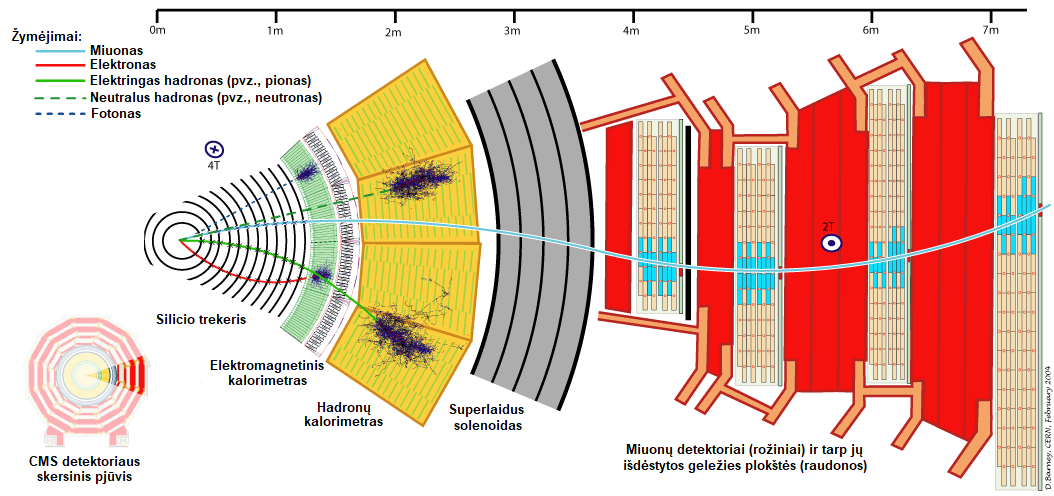
\includegraphics[width=\textwidth]{CMSslice_LT.png}
	\caption{\label{fig:CMSslice}Skersinis CMS detektoriaus pjūvis \cite{CMSslice}.
	Skirtingos linijos žymi įvairių dalelių, išlekiančių iš protonų susidūrimo vietos, trajektorijas.
	Trūki linija žymi elektriškai neutralios dalelės trajektoriją, kuri silicio trekų detektoriuje
	neužfiksuojama.}
\end{figure}

CMS detektoriaus sluoksnius galima pamatyti \ref{fig:CMSslice} paveiksle.
Kiekvienas subdetektorius turi vieną cilindrinę ir dvi antgalių dalis, kurios yra sluoksniškai išdėstytos
aplink protonų susidūrimo vietą.
Kiekvienas subdetektorių sluosknis yra skirtingas ir turi savo paskirtį \cite{CMSexperiment}.

Detektoriaus elektronika nėra pajėgi išsaugoti kiekvieną kas $25$ ns vykstantį įvykį, todėl išsaugomų
įvykių skaičiui sumažinti naudojama dviejų lygių trigerių sistema \cite{CMStrig}.
Pirmojo lygio trigeris -- tai šalia detektoriaus sumontuota specialiai tam sukurta kompiuterinės
įrangos sistema.
Joje realiu laiku minimaliai apdorojami kalorimetrų bei miuonų detektorių duomenys ir pagal juos per
$4 \; \mathrm{\mu s}$ sistema nusprendžia, ar įvykis turėtų būti išsaugomas tolimesnei analizei. 
Pirmojo lygio trigeris išsaugo maždaug $1$ įvykį iš $10000$.
Aukšto lygio trigeris -- tai superkompiuterių sistema, į kurią atkeliauja pirmojo lygio trigerį
aktyvavę įvykiai.
Čia įvykiai atkuriami pasinaudojant pilna detektoriaus užregistruota informacija, naudojami
griežtesni atrankos kriterijai.
Tai padeda įvykių skaičių sumažinti iki maždaug $1000$ įvykių per sekundę.
Pastarieji yra įrašomi ilgalaikiam saugojimui, kad vėliau galėtų būti analizuojami mokslininkų.

Protonų susidūrimo įvykio vaizdas, pasinaudojant detektoriaus užregistruota informacija, atkuriamas naudojantis
dalelių srauto (angl. \textit{Particle Flow}) algoritmu \cite{ParticleFlow}.
Šis algoritmas bando susieti trekų detektoriuje užregistruotus signalus su pataikymais į kalorimetrus arba miuonų
detektorius, taip nustatydamas, kokios dalelės susidarė ir kokie jų parametrai (krūvis, skersinis impulsas,
skersinė energija, pseudosparta ir pan.).
Tokiu būdu gaunamas platus galutinių įvykio produktų sąrašas, leidžiantis pamatyti pilną protonų susidūrimo įvykio vaizdą.

\subsection{Nagrinėjamo proceso signalas ir triukšmas}

Dviejų protonų susidūrimo metu gali įvykti įvairūs procesai (reakcijos).
Drell-Yan proceso metu susidaro du priešingo krūvio leptonai.
Tokia pora gali susidaryti ir kitų procesų metu.
Tai -- \ltq{triukšmo įvykiai}.
Pagrindiniai Drell-Yan proceso triukšmai yra šie: viršūninių kvarkų poros ($t\bar{t}\,$) įvykiai, dviejų bozonų
įvykiai ($WW$, $WZ$ ir $ZZ$), vieno viršūninio kvarko ir $W$ bozono įvykiai ($tW$ arba $\bar{t}W$), $W$ bozono
ir čiurkšlės įvykiai ($\WJets$) bei stipriosios sąveikos nulemti kelių čiurkšlių įvykiai (sutrumpintai vadinami $\QCD$).
Čiurkšlė -- tai daugiausia hadronų (bet taip pat ir kitų dalelių) srautas, gaunamas kvarko arba gliuono hadronizacijos
proceso metu.
Taip pat tiriant Drell-Yan proceso elektronų ir miuonų kanalus vienas iš svarbių triukšmų yra
to paties Drell-Yan proceso taonų kanalas $\DYtau$, kai taonai skyla į elektronus arba miuonus.
Stengiantis išskirti, kokią dalį detektoriaus registruojamuose pasiskirstymuose sudaro signalo (Drell-Yan),
o kokią -- triukšmo įvykiai, yra pasitelkiamas Monte Carlo (MC) modeliavimas ir/arba matavimu grįsti metodai.

Monte Carlo modeliavimas -- tai Monte Carlo metodu sumodeliuoti protonų susidūrimo įvykiai.
Įvykių modeliavimas atliekamas keliais lygmenimis.
Pirmiausia sumodeliuojamas pats protonų susidūrimas ir gaunama, kokios dalelės susidarė jo metu.
Tada modeliuojami po susidūrimo vykstantys antriniai procesai, tokie, kaip hadronizacija, spinduliavimas ir dalelių skilimai.
Galiausiai modeliuojama, kaip įvykio produktai sąveikauja su medžiaga -- detektoriaus komponentais.
Tokį virtualų eksperimentą kartojant daug kartų galima gauti vidutinį rezultatą, kuris yra palyginamas su eksperimentu.
Vis dėlto, sumodeliuoti įvykius taip, kad virtualaus eksperimento sąlygos idealiai atitiktų realaus eksperimento sąlygas,
yra praktiškai neįmanoma.
Norint atsižvelgti į kai kuriuos iš neatitikimų modeliuotiems įvykiams galima pritaikyti tam tikras pataisas.
Tačiau vis tiek egzistuoja neapibrėžtumų, tokių, kaip nepakankamos žinios apie atskirų triukšmo procesų įvykių tikėtinumus,
neidealus detektoriaus atsako modeliavimas, papildomi protonų susidūrimai ir pan., kurie kenkia įverčio kokybei.
Šių problemų gali būti išvengiama triukšmo įvykių skaičiaus įvertinimui naudojant matavimu grįstus metodus.

Matavimu grįsti metodai apjungia matavimą ir modeliavimą, kad būtų gautas kuo tikroviškesnis įvykių skaičiaus įvertis.
Pagrindinis matavimu grįstų įvykių skaičiaus įvertinimo metodų principas remiasi signalo ir kontrolinės sričių apibrėžimais.
Signalo sritis -- tai sritis, pasirinkta taip, kad į ją patektų kuo daugiau signalo ir kuo mažiau triukšmo įvykių.
Kontrolinė sritis -- tai taip pasirinkta sritis, kad į ją patektų kuo daugiau triukšmo ir kuo mažiau signalo įvykių.
Šios dvi sritys turi būti nepersiklojančios.
Skirtingi matavimu grįsti metodai įvairiais būdais transformuoja triukšmo įvykių skaičių, apskaičiuotą kontrolinėje
srityje, į triukšmo įvykių skaičių, patenkantį į signalo sritį.
Eksperimentinėje didelių energijų fizikoje ganėtinai populiarūs yra klaidingo fizikinio objekto atpažinimo ir ABCD metodai.
Jie naudojami įvertinti skaičiui tokių triukšmo įvykių, kurių metu susidarė čiurkšlės.
Triukšmų, siejamų su procesais, kurių metu susidariusios dvi nestabilios dalelės skyla į leptonus nepriklausomai ir su
vienodomis tikimybėmis, indėliui įvertinti naudojamas $\emu$ metodas.
Šiame darbe buvo taikomas $\emu$ metodas bei ruošiamasi klaidingo fizikinio objekto atpažinimo metodo pritaikymui.

\section{Drell-Yan proceso tyrimo metodika}

Šiame skyriuje pristatomi atliktame tyrime naudoti įrankiai bei metodika, supažindinama su jų veikimo principais:
aprašomi naudoti protonų susidūrimų duomenų rinkiniai, juose saugomų užregistruotų įvykių atrankos procedūros,
pritaikytos pataisos bei naudoti arba ketinami naudoti matavimu grįsti Drell-Yan triukšmo įvykių skaičiaus įvertinimo
metodai.
Taip pat trumpai pristatomos paklaidų įvertinimo procedūros.

\subsection{Duomenų rinkiniai}

Šiame darbe buvo naudojami dalinai apdoroti CERN CMS detektoriaus 2016 metais užregistruoti $13$ TeV
energijos protonų susidūrimų duomenys, atitinkantys $35.9$ \invfb integruotąjį šviesį, arba maždaug
$2 \cdot 10^{15}$ protonų susidūrimų.
Tai yra virš $10$ kartų daugiau įvykių, nei užregistruota $2015$-aisiais metais \cite{DY2018}.

Taip pat darbe buvo naudojami modeliuoto Drell-Yan signalo bei pagrindinių triukšmo procesų duomenų rinkiniai.
Drell-Yan signalo bei $\WJets$ proceso duomenų rinkiniai buvo sumodeliuoti naudojant
\textsc{MadGraph5\_aMC@NLO} įvykių modeliavimo programą \cite{MG_aMCatNLO}.
Viršūninio-antiviršūninio kvarko poros ($t\bar{t}\,$) ir vieno viršūninio kvarko kartu su $W$ bozonu ($tW$ arba
$\bar{t}W$) įvykiai buvo sumodeliuoti naudojant \textsc{Powheg} \cite{powheg_ttbar, powheg_tW}.
Visi išvardinti procesai buvo sumodeliuoti pirmos eilės perturbacijų tikslumu (angl. \textit{next-to-leading order} -- NLO).
Dviejų bozonų ($WW$, $WZ$, $ZZ$) įvykiai buvo sumodeliuoti su \textsc{Pythia8} nulinės eilės perturbacijų tikslumu
(angl. \textit{leading order} -- LO) \cite{pythia82}.
Detektoriaus atsakas į kiekvieną iš sumodeliuotų įvykių buvo modeliuojamas naudojantis \textsc{Geant4} programa
\cite{geant4}.

Šiam darbui naudoti CMS Drell-Yan tyrimo grupės dalinai atrinkti duomenys saugomi Pietų Korėjos Tier3 duomenų centre ir užima apie $14$ TB.
Duomenų išdėstymo struktūra schematiškai pavaizduota \ref{fig:duomSchem} pav.
Saugomi duomenys yra skirstomi į modeliuotus ir užregistruotus CMS detektoriumi.
CMS detektoriumi užregistruoti duomenys yra skirstomi į pirminius duomenų rinkinius pagal pirmo lygio trigerio
suveikimą, o pirminiai duomenų rinkiniai dar smulkiau skirstomi pagal duomenų registravimo laikotarpį.
Modeliuoti duomenys yra skirstomi pagal tai, kokio proceso įvykiai yra sumodeliuoti ir, kai kuriais atvejais,
dar yra smulkinami pagal tam tikrus įvykių parametrus (pavyzdžiui, įvykio metu sukurtos dalelės invariantinę masę,
skersinį impulsą ir pan.).
Kai kurie modeliuoti duomenų rinkiniai turi po keletą versijų arba plėtinių.
Duomenų analizei buvo rašomi C++ programiniai moduliai.

\begin{figure}[H]
	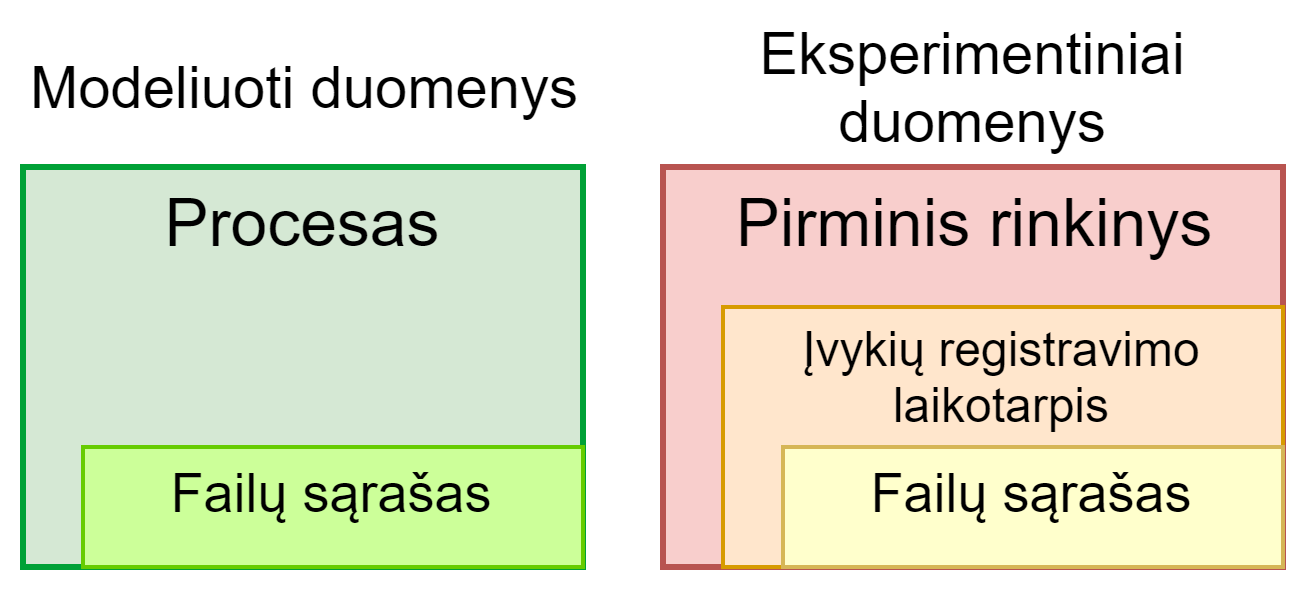
\includegraphics[width=0.7\textwidth]{Duomenu_schema_DataMC_v2.png}
	\caption{\label{fig:duomSchem} Duomenų saugojimo schema.}
\end{figure}

\begin{figure}[H]
	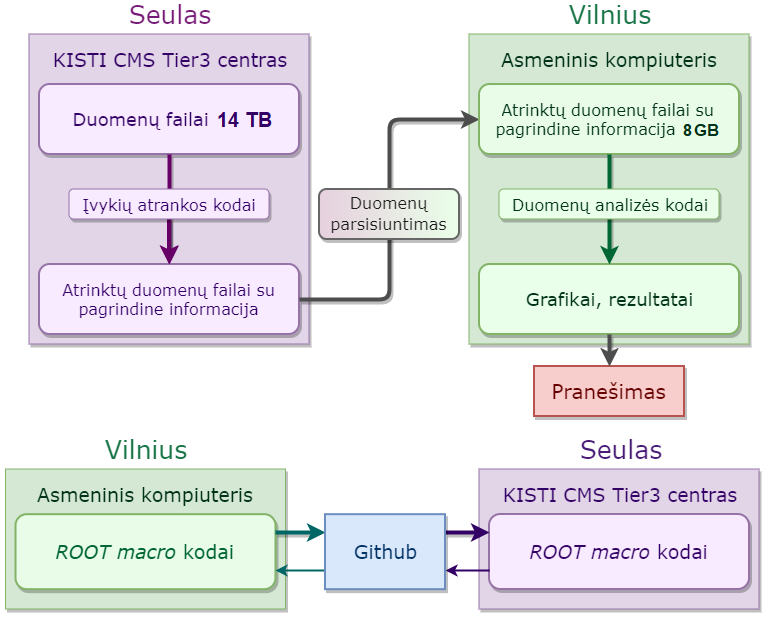
\includegraphics[width=0.9\textwidth]{Duomenu_panaudojimo_schema.png}
	\captionof{figure}{\label{fig:duomVald} Duomenų panaudojimo (viršuje) ir kompiuterinio kodo versijų valdymo (apačioje) schemos.}
\end{figure}

\begin{figure}[H]
	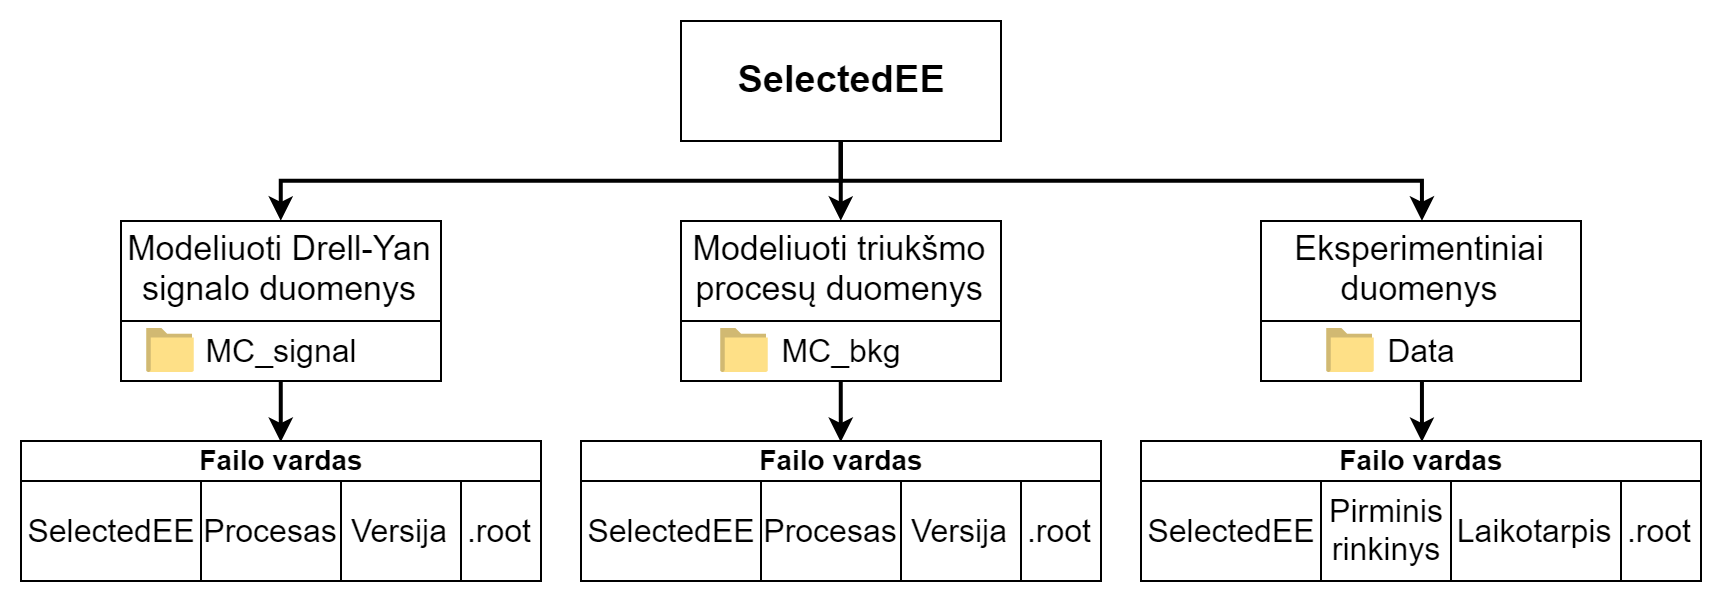
\includegraphics[width=\textwidth]{atrinktu_duomenu_schema_v1.png}
	\captionof{figure}{\label{fig:selectedX} Atrinktų duomenų loginė schema.}
\end{figure}

Duomenų analizė vykdyta dviem etapais: pirmiausia buvo atliekama išmatuotų ir modeliuotų įvykių atranka nuotoliniu
būdu prisijungus prie skaičiavimo centro.
Svarbiausia su atrinktais įvykiais susijusi informacija buvo įrašoma į naujus duomenų failus, kurie užima tik
apie $8$ GB.
Naujai sukurti failai buvo parsisiunčiami į vietinį kompiuterį tolimesnei analizei.
Programinio kodo versijos buvo tvarkomos naudojantis \textit{Github} versijų valdymo sistema.
Apibendrintos duomenų naudojimo ir kodo versijų valdymo schemos yra pavaizduotos \ref{fig:duomVald} pav.
Sumažinti duomenų rinkiniai buvo skirstomi pagal tai, kokios galutinės būsenos įvykiai juose yra saugomi
($ee$, $\mu\mu$, ar $\emu$), tada pagal tai, ar įvykiai yra užregistruoti CMS detektoriumi, ar tai yra modeliuotas
Drell-Yan signalas, ar modeliuotas triukšmas.
Galiausiai atrinkti eksperimentinių duomenų failai buvo išskirstyti pagal pirmojo lygio trigerį ir įvykių
registravimo laikotarpį, o modeliuoti duomenų failai -- pagal procesą (bei, kai kuriais atvejais, tam tikrus
jo parametrus) ir failų versijas.
Atrinktų $ee$ galutinės būsenos duomenų rinkinių loginį išplanavimą galima pamatyti \ref{fig:selectedX} pav.


\subsection{Įvykių atranka}\label{sec:selection}
Iš $2016$-aisiais metais CMS detektoriaus užregistruotų duomenų buvo stengiamasi išrinkti tokius įvykius, kurie
su kuo didesne tikimybe atitiktų Drell-Yan procesą.
Atrankos kriterijai yra apibendrinti \ref{table:selection} lentelėje.

Drell-Yan proceso miuonų galutinei būsenai buvo naudojamas vieno miuono trigeris, kuris aktyvuojamas tada,
kai aptinkamas bent vienas miuonas su skersiniu impulsu, didesniu nei $24$ GeV.
Miuonas turi būti atpažintas pasinaudojant trekų detektoriaus ir miuonų detektorių informacija.
Toliau kiekvienam miuonui buvo taikomi \ttt{TightID} reikalavimai \cite{MuonID}, kurie skirti sumažinti atranką
praeinančių netikrų miuonų, bei miuonų, atsiradusių iš antrinių procesų, skaičių.
\ttt{TightID} reikalavimus atitinka virš $95\%$ protonų susidūrimų metu sukurtų tikrų ir mažiau nei $0.3\%$ netikrų
miuonų \cite{MuonID}.
Taip pat kiekvienam miuonui buvo taikomas trajektorijos izoliuotumo reikalavimas: pašalinių dalelių, aptiktų
$\Delta R = \sqrt{(\Delta\eta)^2 + (\Delta\phi)^2} < 0.3$ (čia $\eta$ -- pseudosparta, $\phi$ -- sferinės koordinačių
sistemos azimutinis kampas) pločio kūgyje, nubrėžtame aplink miuono trajektoriją, skersinių impulsų suma negali
viršyti $15\%$ miuono skersinio impulso vertės: $I_{\mathrm{PF}}^{\mathrm{rel.}}<0.15$ (čia \ltq{PF} žymi tai, jog
šį dydį apskaičiuoja dalelių srauto algoritmas).
Tolimesnis kriterijus buvo toks, kad miuonų poros trajektorijas pakankamai tiksliai eitų suvesti į vieną pirminę
viršūnę bei kad abu miuonai būtų priešingų elektrinių krūvių.
Tam, kad būtų išvengta miuonų iš kosminės spinduliuotės aptikimo, buvo taikomas papildomas kriterijus, reikalaujantis,
kad plokštuminis kampas tarp dviejų miuonų trajektorijų būtų mažesnis, nei $\pi-0.005$ rad.


\begin{table}
	\begin{tabular}{|c|c|}
		\hline
		\textbf{$ee$ įvykiai} & \textbf{$\mu\mu$ įvykiai} \\
		\hline\hline
		\multirow{4}{17em}{\centering Trigeris:\\ \ttt{HLT\_Ele23\_Ele12\_CaloIdL\_} \ttt{TrackIdL\_IsoVL\_DZ}}
			& \multirow{4}{17em}{\centering Trigeris:\\ \ttt{HLT\_IsoMu24} arba \ttt{HLT\_IsoTkMu24} \\ Bent vienas miuonas turi būti aktyvavęs trigerį} \\
		 & \\
		 & \\
		 & \\
		\hline
		\multicolumn{2}{|c|}{$p_{\mathrm{\,1T}} > 28$ GeV, $p_{\mathrm{\,2T}} > 17$ GeV} \\
		\hline
		$|\eta_{\mathrm{SC}}| < 2.4$, & \multirow{2}{17em}{\centering $|\eta| < 2.4$} \\
		\textbf{išskyrus} $1.4442<|\eta_{\mathrm{SC}}|<1.566$ & \\
		\hline
		\ttt{MediumID} reikalavimai & \ttt{TightID} reikalavimai, $I_{\mathrm{PF}}^{\mathrm{rel.}}<0.15$ \\
		\hline
		\multirow{5}{17em}{\centering Atranką turi praeiti lygiai 2 elektronai} &
			\multirow{3}{17em}{\centering Pasirenkami 2 miuonai, kuriuos galima tiksliausiai suvesti į vieną pirminę viršūnę su $\chi^2<20$,} \\
		 & \\
		 & \\ \cline{2-2}
		 & Priešingi elektriniai krūviai, \\ \cline{2-2}
		 & Plokštuminis kampas $< \pi - 0.005$ rad \\
		\hline
	\end{tabular}
	\caption{\label{table:selection}Apibendrinti atrankos kriterijai, taikyti $ee$ ir $\mu\mu$ įvykiams. $p_{\mathrm{\,1T}}$ ir
	$p_{\mathrm{\,2T}}$ žymi greitesniojo ir lėtesniojo leptono skersinį impulsą.
	$\eta_{\mathrm{SC}}$ žymi elektromagnetinio kalorimetro segmento, į kurį pataikė elektronas, pseudospartą.}
\end{table}

Elektronų galutinei būsenai buvo naudojamas dviejų elektronų trigeris, kuris aktyvuojamas tada, kai aptinkami
bent du elektronai, vieno iš kurių skersinis impulsas didesnis, nei $23$ GeV, o kito -- didesnis nei $12$ GeV.
Kiekvienam elektronui buvo taikomi \ttt{MediumID} reikalavimai (idėja aprašyta \cite{EleID}, tačiau tikslios
reikalavimų vertės skiriasi nuo naudotų darbe, nes jos yra atnaujinamos CMS vidiniuose dokumentuose), kurie
skirti sumažinti elektronų, atsiradusių fotono virsmo į elektrono-pozitrono porą metu, bei netikrų elektronų
skaičių.
\ttt{MediumID} reikalavimus atitinka virš $80\%$ protonų susidūrimų metu sukurtų tikrų ir mažiau nei $3.5\%$ netikrų
elektronų \cite{EleID}.
Taip pat buvo reikalaujama, kad elektronai nepatektų į sritį $1.4442<|\eta_{\mathrm{SC}}|<1.566$, nes joje
yra perėjimas iš elektromagnetinio kalorimetro cilindrinės į antgalio dalį ir dėl ten išvedžiotos elektronikos
detektavimo efektyvumas šioje srityje nėra toks geras.

Galiausiai tiek elektronai, tiek miuonai turėjo praeiti tokius pačius kinematinius atrankos kriterijus,
reikalaujančius, kad greitesnysis leptonas turėtų skersinį impulsą, didesnį už $28$ GeV, o lėtesnysis --
didesnį už $17$ GeV bei kad abiejų leptonų pseudospartų absoliutinės vertės neviršytų $2.4$.
Jei tokią atranką praeitų kelios miuonų poros, iš jų išrenkama ta pora, kurios miuonų trajektorijas galima suvesti į
vieną pirminę viršūnę didžiausiu tikslumu.

Pagrindinis matuojamas dydis buvo atranką praėjusių leptonų porų invariantinė masė.
Iš jų verčių buvo brėžiama invariantinės masės histograma, apimanti masės sritį nuo $15$ iki $3000$ GeV.

\subsection{Pataisos}\label{sec:corrections}
CMS eksperimento matavimo rezultatų interpretavimui pasitelkiami modeliuoti protonų susidūrimai.
Matavime užregistruotų įvykių skaičius yra fiksuotas ir nulemtas integruotojo šviesio bei skirtingų
procesų reakcijų skerspjūvių.
Modeliuotų įvykių skaičius gali būti įvairus ir bendru atveju nesutampa su eksperimente užregistruotu
įvykių skaičiumi.
Kad būtų galima palyginti matavimą su modeliavimu, modeliuotų įvykių skaičius turi būti sunormuotas
į išmatuotą integruotąjį šviesį.
Tai daroma kiekvienam modeliuotam įvykiui priskiriant normuojantį svorį $\omega_{i}^{\mathrm{Norm.}}$,
kuris apskaičiuojamas pagal tokią formulę:
\begin{equation}
	\omega_{i}^{\mathrm{Norm.}} = \omega_{i}^{\mathrm{Gen.}} \frac{ \sigma\Lumi }{ \sum_{i=j}^{N}\omega_{j}^{\mathrm{Gen.}} } \; ,
	\label{eq:NLOweight}
\end{equation}
čia $\omega_{i}^{\mathrm{Gen.}}$ kiekvieno įvykio individualus svoris, priskirtas įvykių modeliavimo programos,
$\sigma$ -- tam tikro proceso (pvz., Drell-Yan) teorinis reakcijos skerspjūvis, $N$ -- įvykių skaičius to
proceso modeliuotų duomenų rinkinyje, $\Lumi$ -- išmatuotas integruotasis šviesis.
Daugumos procesų $\omega_{i}^{\mathrm{Norm.}}<1$.

Įprastai per vieną protonų spindulio paketų prasikeitimą (angl.\ \textit{bunch crossing}) susiduria
ne viena, o kelios ar net keliasdešimt protonų porų.
Tai turi įtakos užregistruoto įvykio atkūrimo kokybei.
Šį efektą bandoma simuliuoti modeliuotuose įvykiuose, tačiau dažniausiai tikimybinis protonų susidūrimų
skaičiaus (per vieną prasikeitimą) pasiskirstymas matavime ir modeliavime nesutampa.
Tai siejasi su atsitiktinėmis susidūrimų fliuktuacijmis, o taip pat ir su Didžiojo hadronų greitintuvo
technikų tyrinėjimais keičiant protonų spindulio intensyvumą, paketų skaičių, spindulio persiklojimo
tūrį ir pan.
Šį nesutapimą bandoma sumažinti taikant protonų susidūrimo skaičiaus pataisas -- kiekvienam modeliuotam
įvykiui priskiriamas tam tikras papildomas svoris pagal tai, koks protonų susidūrimų skaičius jame buvo sumodeliuotas.
Pataisa buvo taikoma darant prielaidą, kad protonų susidūrimo skerspjūvis greitintuve yra lygus $64$ mb
($6.4 \cdot 10^{-30} \, \mathrm{m}^2)$.

Elektronų poros invariantinės masės matavimo kokybei ženklios įtakos turi elektronų energijos matavimo
tikslumas, o miuonų poros invariantinei masei -- miuonų skersinio impulso matavimo tikslumas.
Dėl to visiems užregistruotiems elektronams buvo pritaikytos standartinės CMS elektronų energijos skalės
pataisų procedūros \cite{Ecorr}, o miuonams -- Ročesterio mokslinės grupės pateikiamos miuonų impulso
skalės pataisos \cite{RocCorr}.

Dėl modeliavimo netobulumo nesutapo tam tikros realaus ir virtualaus eksperimento sąlygos, todėl
kiekvienam elektronų poros įvykiui buvo priskiriami svoriniai daugikliai, priartinantys modeliuotus trigerių
suveikimo ir elektrono trajektorijos atkūrimo bei atpažinimo efektyvumus prie išmatuotųjų verčių.
Miuonų poros įvykiams buvo priskirti daugikliai, atsižvelgiantys į trigerių bei miuonų trajektorijos atkūrimo,
atpažinimo ir izoliuotumo įvertinimo efektyvumų nesutapimus.
Kiekvieno suvidurkinto daugiklio vertė buvo nustatoma pagal leptono skersinio impulso ir pseudospartos vertes.
Tipinė daugiklio vertė yra apie $0.9$.

Yra pastebėta, kad pirmos eilės perturbacijų tikslumu modeliuojant viršūninių kvarkų poros ($t\bar{t}\,$)
įvykius, gaunami modeliuoti viršūninių kvarkų skersinių impulsų pasiskirstymai turi nesutapimų su nustatytaisiais
eksperimentiškai \cite{ttbarPT}.
Kadangi $t\bar{t}$ yra vienas iš Drell-Yan triukšmo procesų, norint turėti kuo tikslesnį triukšmo įvertį, į šį
modeliavimo trūkumą svarbu atsižvelgti.
Tai buvo daroma modeliuotiems viršūninių kvarkų poros įvykiams priskiriant papildomus svorius, kurie skirti
priartinti modeliuotą kvarkų skersinių impulsų pasiskirstymą prie naujausių eksperimentinių rezultatų.
Svorių vertės nustatomos pagal kvarkų skersinių impulsų $p_{\mathrm{T}}^{t}$ vertes.
Tipinės svorių vertės yra didesnės už $1$, kai abiejų kvarkų $p_{\mathrm{T}}^{t}<123 \, \mathrm{GeV}$, ir mažesnės už $1$,
kai $p_{\mathrm{T}}^{t}>120 \, \mathrm{GeV}$.

Neidealios eksperimentinės sąlygos nulemia matavimo ir modeliavimo rezultatų nesutapimą.
Dvi aplinkybės paveikė leptonų poros spartos pasiskirstymus.
Į tai atsižvelgti modeliuotiems įvykiams buvo pritaikytos dvi pataisos.
Viena pataisa buvo skirta ištaisyti protonų susidūrimo vietos $z$ koordinatės ($z$ ašis eina išilgai protonų
spindulio lėkimo krypties detektoriaus centre) nesutapimą tarp matavimo ir modeliavimo.
Antroji pataisa buvo reikalinga todėl, kad darbe naudotų duomenų registravimo laikotarpiu buvo susidurta su problema,
kai tam tikru atveju trigerio suveikimas buvo priskiriamas ne tam įvykiui, kuris iš tikrųjų jį aktyvavo, o
ankstesniam.
Dėl šio efekto dalis įdomių įvykių, kuriuose sukurtos dalelės turėjo dideles pseudospartos vertes ($|\eta|>2$)
liko neįrašyti.
Imituoti šiam pernelyg ankstyvo trigerio suveikimo efektui buvo pritaikyta pataisa, kuri priskirdavo įvykiams
svorius pagal tai, kiek ir kokių įvykyje užregistruotų objektų patenka į didesnių pseudospartų sritį.
Tipinės pataisų vertės vienam įvykiui siekė apie $0.98$ ir mažiau įvykiams, kuriuose buvo užfiksuoti objektai su
$|\eta|>2$.

\subsection{Matavimu grįsti triukšmo įvykių skaičiaus įvertinimo metodai}
Matavimu grįstų metodų esmė -- nustatyti triukšmo įvykių skaičių kontrolinėje srityje, kurioje dominuoja triukšmas
ir gautą rezultatą transformuoti į signalo sritį, kuri yra tiriama.
Toliau pateikiami $\emu$ metodo ir klaidingo fizikinio objekto atpažinimo metodo veikimo principų aprašymai.
$\DYtau$, $t\bar{t}\,$, $WW$, $tW$ ir $\bar{t}W$ triukšmo procesų indėlis buvo įvertintas $\emu$ metodu.
$\WZ$ ir $\ZZ$ įvykių skaičius buvo įvertintas iš modeliavimo.
Kol kas $\WJets$ įvykių skaičius taip pat buvo įvertintas iš modeliavimo, o $\QCD$ įvykių skaičius modeliavimu yra
aprašomas labai nekokybiškai, todėl kol kas į tyrimą nebuvo įtrauktas.
Tikslesniam $\WJets$ ir $\QCD$ procesų indėlio įvertinimui tolimesniame darbe ketinama pritaikyti fizikinio objekto klaidingo
atpažinimo metodą.

\subsubsection{$\emu$ metodas}\label{sec:SignalBkg}

$\emu$ metodas yra tinkamas įvertinti triukšmo įvykių skaičiui tokių procesų, kurių metu susidaro dvi
nestabilios dalelės, galinčios nepriklausomai skilti į vienodų arba skirtingų rūšių leptonus.
Tokio proceso pavyzdys yra $W^{\!+}\!W^{\!-}$ procesas.
Nagrinėjant tik leptoninius skilimus bei atmetant skilimą į taonus ir nekreipiant dėmesio į skilimo metu
susidarančius neutrinus, kurie CMS detektoriuje yra neaptinkami,
galimos tokios įvykio baigtys: $WW\!\!\rightarrow\! e^{\!+}\! e^{\!-}$, $WW\!\!\rightarrow\! e^{\!+}\!\mu^{\!-}$,
$WW\!\!\rightarrow\! \mu^{\!+}\!e^{\!-}$, $WW\!\!\rightarrow\! \mu^{\!+}\!\mu^{\!-}$.
Taikant $\emu$ metodą signalo sritis -- $ee$ arba $\mu\mu$ įvykiai -- apibrėžiama pagal \ref{sec:selection} skyriuje
aprašytus kriterijus.
Kontrolinė sritis apibrėžiama pagal panašius kriterijus, tačiau galutinėje būsenoje ieškoma
ne dviejų elektronų ar dviejų miuonų, o vieno elektrono ir vieno miuono.
Tai -- $\emu$ įvykiai.
Tokios būsenos neįmanoma gauti iš Drell-Yan proceso signalo, taigi joje bus vien triukšmas.
Triukšmo įvykių skaičius iš kontrolinės srities ($\emu$) į signalo sritį ($ee$ arba $\mu\mu$)
transformuojamas pasinaudojant Monte Carlo modeliavimo rezultatais:

\begin{equation}
	N_{ee}^{\mathrm{Tr. \, įvert.}} =
	\frac{ N_{ee}^{\mathrm{Tr. \, MC}} }{ N_{e\mu}^{\mathrm{Tr. \, MC}} }
	\cdot N_{e\mu}^{\mathrm{Tr. \, eksp.}} \; ,
	\label{eq:emuMethod}
\end{equation}
čia $N_{ee}^{\mathrm{Tr. \, įvert.}}$ -- $\emu$ metodu įvertintas triukšmo įvykių skaičius signalo
(šiuo atveju, $ee$) srityje, $N_{e\mu}^{\mathrm{Tr. \, eksp.}}$ -- išmatuotas įvykių skaičius
kontrolinėje srityje, $N_{ee}^{\mathrm{Tr. \, MC}}$ ir $N_{e\mu}^{\mathrm{Tr. \, MC}}$ -- modeliuotų
triukšmo įvykių skaičiai atitinkamai signalo ir kontrolinėje srityje.

Elektrono ir miuono galutinės būsenos įvykiai buvo atrenkami kombinuojant $ee$ ir $\mu\mu$ atrankos
kriterijus -- elektronui buvo taikomi $ee$ atrankoje naudoti, o miuonui -- $\mu\mu$ atrankoje naudoti
kriterijai, tik šiai atrankai buvo naudotas vieno miuono trigeris (nenaudota elektronų trigerių).
Apibendrinti $e\mu$ įvykių atrankos kriterijai pateikiami \ref{table:emusel} lentelėje.
Šiems įvykiams buvo pritaikytos ir visos \ref{sec:corrections} skyriuje aprašytos pataisos.

\vspace{0.5cm}
\begin{table}[H]
	\begin{tabular}{|c|c|}
		\hline
		\centering \textbf{Elektronas} & \textbf{Miuonas} \\
		\hline\hline
		\multicolumn{2}{|c|}{\centering Trigeris \ttt{HLT\_IsoMu24} arba \ttt{HLT\_IsoTkMu24}} \\
		\multicolumn{2}{|c|}{\centering Atrinktas miuonas turi būti tas, kuris aktyvavo trigerį} \\
		\hline
		\multicolumn{2}{|c|}{\centering $p_{\mathrm{\,1T}} > 28$ GeV, $p_{\mathrm{\,2T}} > 17$ GeV} \\
		\hline
		\multirow{2}{17em}{\centering $|\eta_{\mathrm{SC}}| < 2.4$,\\ \textbf{išskyrus} $1.4442<|\eta_{\mathrm{SC}}|<1.566$} &
			\multirow{2}{17em}{\centering $|\eta| < 2.4$} \\
		 & \\
		\hline
		\ttt{MediumID} reikalavimai & \ttt{TightID} reikalavimai, $I_{\mathrm{PF}}^{\mathrm{rel.}}<0.15$ \\
		\hline
		\multicolumn{2}{|c|}{\multirow{2}{34em}{\centering Pasirenkamos 2 dalelės ($e$ ir $\mu$), kurias galima tiksliausiai suvesti į vieną pirminę viršūnę su $\chi^2<20$,}} \\
		\multicolumn{2}{|c|}{} \\
		\hline
		\multicolumn{2}{|c|}{\centering Plokštuminis kampas $< \pi - 0.005$ rad} \\
		\hline
		\multicolumn{2}{|c|}{\centering \textbf{Priešingi elektriniai krūviai} -- $\emu$ metodui,} \\
		\multicolumn{2}{|c|}{\centering \textbf{vienodi krūviai} -- $\emu$ $\QCD$ įvertinimui}\\
	\hline
	\end{tabular}
	\caption{\label{table:emusel}Apibendrinti atrankos kriterijai, taikyti elektronui ir miuonui $\emu$ įvykių atrankoje.
	$p_{\mathrm{\,1T}}$ ir $p_{\mathrm{\,2T}}$ žymi greitesniojo ir lėtesniojo leptono skersinį impulsą,
	$\eta_{\mathrm{SC}}$ žymi elektromagnetinio kalorimetro segmento, į kurį pataikė elektronas, pseudospartą, o
	$I_{\mathrm{PF}}^{\mathrm{rel.}}$ -- miuono trajektorijos izoliuotumą.}
\end{table}

$\WJets$ ir $\QCD$ įvykių metu susidariusi čiurkšlė gali būti klaidingai atpažinta kaip leptonas, todėl
$\emu$ įvykių atranką praeina ir ganėtinai reikšminga netikrų $\emu$ įvykių dalis.
Norint kaip įmanoma tiksliau įvertinti Drell-Yan proceso triukšmo įvykių skaičių, svarbu atliekant skaičiavimus atsižvelgti
į tokių įvykių egzistavimą.
$\QCD$ indėlis buvo įvertintas dar vienu matavimu grįstu metodu.
Šiuo atveju signalo sritis jau yra $\emu$ įvykiai, kuriuose elektronas ir miuonas yra priešingų elektrinių
krūvių, o kontrolinė sritis -- įvykiai, kuriuose elektrono ir miuono krūviai yra vienodi.
$\QCD$ įvykių skaičiaus įvertinimo principas yra pavaizduotas \ref{fig:emuQCD} pav.
Kairiajame grafike matomas didžiulis skirtumas tarp eksperimentinio ir modeliuoto rezultato buvo
priskirtas su $\QCD$ procesu siejamiems netikriems $\emu$ įvykiams.
$\QCD$ įvykių skaičius iš vienodų krūvių (kontrolinės) srities į priešingų krūvių (signalo) sritį
buvo transformuotas padalinus jį iš konstantos $R\approx 0.57$, kuri apskaičiuojama teoriškai,
padarius prielaidą, kad visi atranką praeinantys $\QCD$ įvykiai yra gelminių kvarkų poros
($b\bar{b}$) įvykiai.
Lyginant su ankstesniu darbu \cite{MAk1}, ši metodika buvo patobulinta įtraukiant su $\WJets$ procesu siejamus netikrus $\emu$ įvykius.
Su $\WJets$ procesu siejamų netikrų $e\mu$ įvykių skaičius buvo įvertintas iš modeliavimo.
Prieš taikant $\emu$ metodą gautas $\QCD$ įvykių skaičiaus įvertis buvo atimtas iš
$N_{e\mu}^{\mathrm{Tr. \, eksp.}}$, o $W+\mathrm{Jets}$ indėlis buvo įskaitytas sumažinant
$N_{e\mu}^{\mathrm{Tr. \, eksp.}}$ dydžiu $1/(1+C)$, kur
\begin{equation*}
	C = \frac{ N_{W+\mathrm{Jets}}^{\mathrm{MC}} } { N_{\mathrm{DY}\rightarrow\tau\tau}^{\mathrm{MC}} + 
	N_{t\bar{t}}^{\mathrm{MC}} + N_{WW}^{\mathrm{MC}} + N_{WZ}^{\mathrm{MC}} + N_{tW}^{\mathrm{MC}} + N_{\bar{t}W}^{\mathrm{MC}} +
	N_{ZZ}^{\mathrm{MC}} } \; ,
\end{equation*}
čia $N^{\mathrm{MC}}_{\mathrm{proc.}}$ -- modeliuotų tam tikro proceso $\emu$ galutinės būsenos įvykių skaičius.

\begin{figure}[H]
	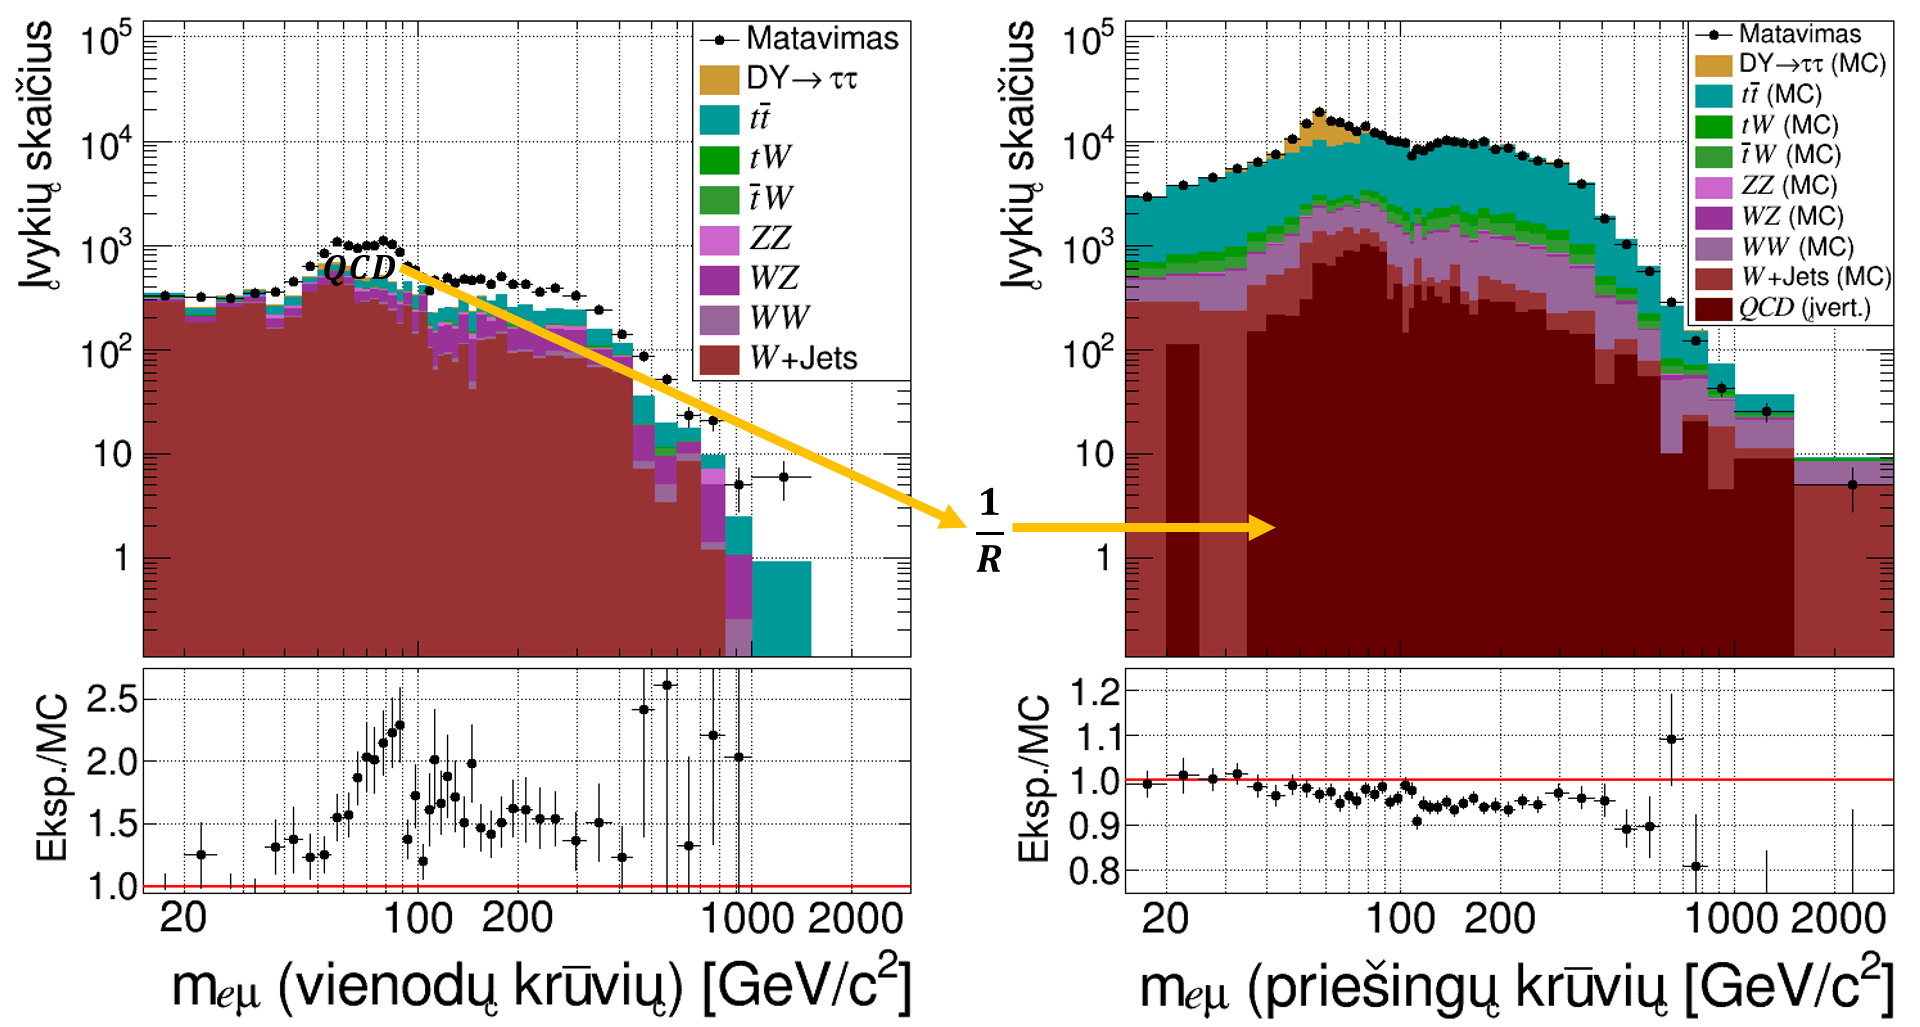
\includegraphics[width=0.95\textwidth]{emuQCDest.png}
	\vspace{-0.2cm}
	\caption{\label{fig:emuQCD} Vienodą (kairėje) ir priešingą (dešinėje) krūvį turinčių elektrono ir
	miuono invariantinės masės pasiskirstymai.
	Rodyklės iliustruoja, kaip buvo įvertinamas netikrų $\emu$ ($\QCD$) įvykių skaičius.
	}
\end{figure}


\subsubsection{Klaidingo atpažinimo metodas}

Fizikinio objekto klaidingo atpažinimo metodas yra naudojamas įvertinti skaičiui tokių triukšmo įvykių, kurie užregistruojami,
kai protonų susidūrimo įvykio atkūrimo algoritmas klaidingai atpažįsta vieną ar kelis fizikinius objektus, pavyzdžiui, kai fotonas
būna klaidingai atpažįstamas kaip elektronas, čiurkšlė -- kaip elektronas arba miuonas ir pan.
Tęsiant šį darbą tikimasi klaidingo atpažinimo metodu įvertinti $\QCD$ ir $\WJets$ triukšmų indėlį.
Klaidingo atpažinimo metodo veikimo principas remiasi tikimybės, kad čiurkšlė bus klaidingai atpažinta kaip kita dalelė,
apskaičiavimu ir pritaikymu triukšmo įvykių skaičiui, įvertintam kontrolinėje srityje, transformuoti į triukšmo įvykių skaičių,
patenkantį į signalo sritį.

Miuonų įvykiams kontrolinė sritis galėtų būti apibrėžiama kaip tokie įvykiai, kuriuose atpažintų miuonų trajektorijų izoliuotumas yra prastas:
reikalaujama, kad visų šalutinių trajektorijų, užfiksuotų $\Delta R < 0.3$ pločio kūgyje, nubrėžtame aplink miuono trajektoriją,
skersinių impulsų suma būtų didesnė už $15\%$ miuono skersinio impulso vertės: $I_{\mathrm{PF}}^{\mathrm{rel.}}>0.15$.
Vykdant įprastą (signalo) įvykių atranką reikalavimas buvo atvirkščias: $15\%$ miuono skersinio impulso vertės negalima viršyti).
Konkrečiau preliminarūs atrankos kriterijai miuonui, patenkančiam į signalo ir kontrolinę sritis pateikiami \ref{table:FR} lentelėje.
Tada klaidingo atpažinimo tikimybė apibrėžiama, kaip procentinė dalis visų čiurkšlių, patenkančių į signalo sritį:
\begin{equation}
	f_{\mathrm{signal} \,| \,\mathrm{Jet}}(\pT, \, \eta) =
	\frac{N^{\QCD}_{\mathrm{signal}}(\pT, \, \eta)}{N^{\QCD}_{\mathrm{signal}}(\pT, \, \eta)+N^{\QCD}_{\mathrm{control}}(\pT, \, \eta)} \; ,
\end{equation}
čia $f_{\mathrm{signal} \,| \,\mathrm{Jet}}(\pT, \, \eta)$ -- tikimybė čiurkšlei, su tam tikru skersiniu impulsu $\pT$ ir pseudosparta $\eta$
patekti į signalo sritį, $N^{\QCD}_{\mathrm{signal}}(\pT, \, \eta)$ -- į signalo srities dalį su konkrečiomis parametrų $(\pT, \, \eta)$
vertėmis patenkančių dalelių, kurios buvo kaip atpažintos, kaip izoliuoti miuonai, tačiau yra kilusios iš $\QCD$ proceso, skaičius,
$N^{\QCD}_{\mathrm{control}}(\pT, \, \eta)$ -- į kontrolinę sritį patenkančių dalelių, kurios buvo kaip atpažintos, kaip neizoliuoti
miuonai ir taip pat yra kilusios iš $\QCD$ proceso, skaičius.
Čia imamas būtent $\QCD$ procesas, nes jo metu susidaro vien tik čiurkšlės -- tai praktiškai garantuoja, kad trajektorija, kurią
algoritmas atkūrė kaip miuono trajektoriją, iš tikrųjų buvo čiurkšlė.
Iš tiesų, miuonas gali susidaryti čiurkšlėje vykstančių hadronizacijos procesų metu, bet toks miuonas neišvengiamai turėtų būti
neizoliuotas.
Taigi, galima daryti prielaidą, kad visos atkurtos izoliuotos miuonų trajektorijos, gautos iš $\QCD$ proceso buvo klaidingai atpažintos.

\begin{table}
	\begin{tabular}{|c|c|}
		\hline
		\textbf{Signalo sritis} & \textbf{Kontrolinė sritis} \\
		\hline\hline
		\multicolumn{2}{|c|}{Trigeris \ttt{Mu\_50}} \\
		\hline
		\multicolumn{2}{|c|}{$\pT>52$ GeV} \\
		\hline
		\multicolumn{2}{|c|}{$|\eta|<2.4$} \\
		\hline
		\multicolumn{2}{|c|}{\ttt{TightID} reikalavimai} \\
		\hline
		$I_{\mathrm{PF}}^{\mathrm{rel.}} < 0.15$ & $I_{\mathrm{PF}}^{\mathrm{rel.}} > 0.15$ \\
		\hline
	\end{tabular}
	\caption{\label{table:FR} Galimi miuonų atrankos kriterijai signalo ir kontrolinei sritims. Visi kriterijai, išskyrus vieną
	abejoms sritims yra vienodi.
	$I_{\mathrm{PF}}^{\mathrm{rel.}}$ žymi miuono trajektorijos izoliuotumą.}
\end{table}

Norint apskaičiuoti klaidingo atpažinimo tikimybę pagrindinė užduotis yra nustatyti su $\QCD$ procesu siejamų įvykių skaičių
$N^{\QCD}_{\mathrm{signal}}(\pT, \, \eta)$ ir $N^{\QCD}_{\mathrm{control}}(\pT, \, \eta)$.
Taip pat, kaip turint vien tik CMS detektoriaus užregistruotus duomenis negalima vienareikšmiškai nustatyti, kuris įvykis yra
sietinas su Drell-Yan procesu, o kuris -- su triukšmo, šiuo atveju irgi neįmanoma tiesiogiai įvertinti, kurie įvykiai yra
sietini su $\QCD$ procesu.
Statistiniam $\QCD$ įvykių skaičiaus įvertinimui galimos trys pagrindinės strategijos:
\begin{enumerate}
	\item Atimties metodas -- $\QCD$ įvykių skaičius įvertinamas iš signalo arba kontrolinės srities atranką praėjusių eksperimentinių
	įvykių skaičiaus atėmus modeliuotą visų su $\QCD$ nesusijusių procesų įvykių skaičių:
	\begin{multline}
		N^{\QCD}_{i, \, \pT, \, \eta} = N^{\mathrm{Data}}_{i, \, \pT, \, \eta} - \left( N^{\mathrm{DY}}_{i, \, \pT, \, \eta} +
		N^{W+\mathrm{Jets}}_{i, \, \pT, \, \eta} +  N^{\ttbar+tW+\tbarW}_{i, \, \pT, \, \eta} +
		N^{WW+WZ+ZZ}_{i, \, \pT, \, \eta} \right)^{\mathrm{MC}}; \\ i = \mathrm{signal}, \, \mathrm{control}.
	\end{multline}
	Čia visur dydžių priklausomybė nuo skersinio impulso ir pseudospartos vietoje žymėjimo tarp skliaustelių, kaip buvo pažymėta anksčiau,
	yra žymima apatiniuose indeksuose.
	\item Santykio metodas -- $\QCD$ įvykių skaičius įvertinamas iš matavimo paėmus procentinę $\QCD$ įvykių dalį, kuri buvo apskaičiuota
	pasinaudojant modeliavimu:
	\begin{multline}
		N^{\QCD}_{i, \, \pT, \, \eta} = N^{\mathrm{Data}}_{i, \, \pT, \, \eta} \cdot \left(\frac{N^{\QCD}_{i, \, \pT, \, \eta}}
		{N^{\QCD}_{i, \, \pT, \, \eta} + N^{\mathrm{DY}}_{i, \, \pT, \, \eta} + N^{W+\mathrm{Jets}}_{i, \, \pT, \, \eta} +
		N^{\ttbar+tW+\tbarW}_{i, \, \pT, \, \eta} N^{WW+WZ+ZZ}_{i, \, \pT, \, \eta}} \right)^{\mathrm{MC}}; \\ i = \mathrm{signal}, \, \mathrm{control}.
	\end{multline}
	\item Šablonų pritaikymo metodas -- $\QCD$ įvykių skaičius įvertinamas prie tam tikro išmatuoto pasiskirstymo pritaikius
	skirtingų procesų pasiskirstymų šablonus, gautus iš modeliavimo.
	Pasiskirstymas, pagal kurį šablonai pritaikomi prie matavimo, turi būti pasirenkamas toks, kuris leistų diskriminuoti tarp
	ieškomo ($\QCD$) ir kitų procesų.
	Pavyzdžiui, miuonų atveju, labai gerai tinkamas yra dalelių srauto algoritmo apskaičiuoto miuono trajektorijos izoliuotumo
	pasiskirstymas.
	Turint išmatuotą ir modeliuotus tam tikro parametro pasiskirstymus, stengiamasi gauti geriausią sutapimą tarp matavimo ir
	modeliavimo varijuojant modeliuotą įvykių skaičių:
%	\begin{multline}
%		N^{\mathrm{Data}}_{i, \, \mathcal{P}, \, \eta} \approx
%		\lambda^{\mathrm{fit}}_{\,i, \, \eta}\, N^{\,\QCD \; \mathrm{MC}}_{i, \, \mathcal{P}, \, \eta} +
%		\epsilon^{\,\mathrm{fit}}_{\,i, \, \eta}\, N^{\,\mathrm{DY} \; \mathrm{MC}}_{i, \, \mathcal{P}, \, \eta} +
%		\zeta^{\,\mathrm{fit}}_{\,i, \, \eta}\, N^{\,W+\mathrm{Jets} \; \mathrm{MC}}_{i, \, \mathcal{P}, \, \eta} +
%		\theta^{\,\mathrm{fit}}_{i, \, \eta}\, N^{\,\ttbar \; \mathrm{MC}}_{i, \, \mathcal{P}, \, \eta} + \\[7pt] +
%		\kappa^{\,\mathrm{fit}}_{\,i, \, \eta}\, N^{\,tW \; \mathrm{MC}}_{i, \, \mathcal{P}, \, \eta} + 
%		\xi^{\,\mathrm{fit}}_{i, \, \eta}\, N^{\,\tbarW \; \mathrm{MC}}_{i, \, \mathcal{P}, \, \eta} +
%		\tau^{\,\mathrm{fit}}_{i, \, \eta}\, N^{\,WW \; \mathrm{MC}}_{i, \, \mathcal{P}, \, \eta} +
%		\chi^{\,\mathrm{fit}}_{\,i, \, \eta}\, N^{\,W\!Z \; \mathrm{MC}}_{i, \, \mathcal{P}, \, \eta} +
%		\psi^{\,\mathrm{fit}}_{i, \, \eta}\, N^{\,Z\!Z \; \mathrm{MC}}_{i, \, \mathcal{P}, \, \eta}; \\ i = \mathrm{signal}, \, \mathrm{control}.
%	\end{multline}
	\begin{equation}
		N^{\mathrm{Data}}_{i, \, \mathcal{P}, \, \eta} \approx \sum_{\mathrm{proc}}
		\lambda^{\mathrm{proc,\, fit}}_{\,i, \, \eta}\, N^{\,\mathrm{proc,\, MC}}_{i, \, \mathcal{P}, \, \eta},
		\;\;\;\; i = \mathrm{signal}, \, \mathrm{control}.
	\end{equation}
%	Čia $\lambda^{\mathrm{fit}}_{\,i, \, \eta}$, $\epsilon^{\,\mathrm{fit}}_{\,i, \, \eta}$ ir t.t.\ -- varijuojami daugikliai,
	Čia $\lambda^{\mathrm{proc,\, fit}}_{\,i, \, \eta}$ -- kiekvienam procesui ($\QCD$, $\WJets$, DY ir t.t.)\ skirtingi varijuojami daugikliai,
	kuriuos keičiant bandoma gauti geriausią modeliuotų pasiskirstymų sumos sutapimą su išmatuotuoju pasiskirstymu.
	Geriausių daugiklių verčių ieškoma mažiausių kvadratų metodu.
	Idealiu atveju šie daugikliai turėtų būti lygūs vienetui. 
	$\mathcal{P}$ -- pasirinktas parametras, kurio modeliuoti pasiskirstymai (šablonai) pritaikomi prie matavimo.
	Miuonų atveju tai galėtų būti $\mathcal{P}=I^{\mathrm{rel.}}_{\mathrm{PF}}$.
	Gavus daugiklių vertes klaidingo atpažinimo tikimybė įvertinama modeliuotus dvimačius skersinio impulso ir pseudospartos pasiskirstymus,
	padauginant iš gautųjų daugiklių verčių:
	\begin{equation}
		f_{\mathrm{signal} \,| \,\mathrm{Jet}}(\pT, \, \eta) =
		\frac{\lambda^{\QCD,\,\mathrm{fit}}_{\,\mathrm{signal}, \, \eta}\, N^{\,\QCD \; \mathrm{MC}}_{\mathrm{signal}, \, \pT, \, \eta}}
		{\lambda^{\QCD,\,\mathrm{fit}}_{\,\mathrm{signal}, \, \eta}\, N^{\,\QCD \; \mathrm{MC}}_{\mathrm{signal}, \, \pT, \, \eta} +
		\lambda^{\QCD,\,\mathrm{fit}}_{\,\mathrm{control}, \, \eta}\, N^{\,\QCD \; \mathrm{MC}}_{\mathrm{control}, \, \pT, \, \eta}}\, .
	\end{equation}
	Šablonų pritaikymo metodas yra laikomas tiksliausiu iš trijų išvardintų.
\end{enumerate}

Apskaičiavus klaidingo atpažinimo tikimybę galima ją pritaikyti įvertinant, koks kiekis klaidingai atpažintų dalelių galėjo patekti į signalo
sritį.
Tyrinėjant Drell-Yan procesą kiekviename įvykyje yra ieškoma dviejų elektronų arba dviejų miuonų, todėl reikia įvertinti ir tuos atvejus, kai
klaidingai atpažintas buvo vienas leptonas, ir kai klaidingai atpažinti buvo abu.
Bendrai, pilnas Drell-Yan proceso atranką praėjusių (į signalo sritį patenkančių) įvykių skaičius gali būti išreikštas taip:
%\begin{multline}
%	\label{eq:realfake}
%	N_{\mathrm{signal, \; signal}}(p_{\mathrm{T}\, 1}, \, \eta_{\, 1}, \, p_{\mathrm{T}\, 2}, \, \eta_{\, 2}) =
%	N_{l, \, l}(p_{\mathrm{T}\, 1}, \, \eta_{\, 1}, \, p_{\mathrm{T}\, 2}, \, \eta_{\, 2}) \cdot 
%	f_{\mathrm{signal} \,| \,\mu}(p_{\mathrm{T}\, 1}, \, \eta_{\, 1}) \cdot f_{\mathrm{signal} \,| \, l}(p_{\mathrm{T}\, 2}, \, \eta_{\, 2}) + \\[5pt] +
%	N_{l, \, \mathrm{Jet}}(p_{\mathrm{T}\, l}, \, \eta_{\, l}, \, p_{\mathrm{T}\, \mathrm{Jet}}, \, \eta_{\, \mathrm{Jet}}) \cdot 
%	f_{\mathrm{signal} \,| \, l}(p_{\mathrm{T}\, l}, \, \eta_{\, l}) \cdot
%	f_{\mathrm{signal} \,| \,\mathrm{Jet}}(p_{\mathrm{T \, Jet}}, \, \eta_{\,\mathrm{Jet}}) + \\[5pt] +
%	N_{\mathrm{Jet, \, Jet}}(p_{\mathrm{T}\, 1}, \, \eta_{\, 1}, \, p_{\mathrm{T}\, 2}, \, \eta_{\, 2}) \cdot 
%	f_{\mathrm{signal} \,| \,\mathrm{Jet}}(p_{\mathrm{T}\, 1}, \, \eta_{\, 1}) \cdot
%	f_{\mathrm{signal} \,| \,\mathrm{Jet}}(p_{\mathrm{T}\, 2}, \, \eta_{\, 2})\, ,
%\end{multline}
\begin{multline}
	\label{eq:realfake}
	N_{\mathrm{signal, \; signal}}(p_{\,\mathrm{1T}}, \, \eta_{\, 1}, \, p_{\,\mathrm{2T}}, \, \eta_{\, 2}) =
	N_{l_1, \, l_2} \cdot 
	f_{\mathrm{signal} \,| \,l_1} \cdot f_{\mathrm{signal} \,| \, l_2} +
	N_{l, \, \mathrm{Jet}} \cdot 
	f_{\mathrm{signal} \,| \, l} \cdot f_{\mathrm{signal} \,| \,\mathrm{Jet}} + \\ +
	N_{\mathrm{Jet_1, \, Jet_2}} \cdot 
	f_{\mathrm{signal} \,| \,\mathrm{Jet_1}}\cdot f_{\mathrm{signal} \,| \,\mathrm{Jet_2}}\, ,
\end{multline}
čia $l$ žymi tikrą leptoną ir gali būti $e$ arba $\mu$, $N_{l_1, \, l_2}$, $N_{l, \, \mathrm{Jet}}$, $N_{\mathrm{Jet_1, \, Jet_2}}$ -- įvykių,
kurių metu susidarė atitinkamai du leptonai, leptonas ir čiurkšlė, arba dvi čiurkšlės, skaičius, priklausantis nuo fazinės erdvės, į kurią patenka
nagrinėjami fizikiniai objektai, srities $(p_{\,\mathrm{1T}}, \, \eta_{\, 1}, \, p_{\,\mathrm{2T}}, \, \eta_{\, 2})$.
$f_{\mathrm{signal} \,| \,\mathrm{Jet}}$ -- klaidingo atpažinimo tikimybė fazinės erdvės srityje $(p_{\mathrm{\, Jet \, T}}, \, \eta_{\,\mathrm{Jet}})$. $f_{\mathrm{signal} \,| \,l}$ -- tikimybė, kad tikras leptonas, patenkantis į tam tikrą fazinės erdvės sritį $(p_{\, l\, \mathrm{T}}, \, \eta_{\, l})$ bus
teisingai atpažintas (dar vadinama efektyvumu).
\eqref{eq:realfake} lygybės dešinė pusė susideda iš trijų dėmenų.
Pirmasis dėmuo yra siejamas su tikrų leptonų įvykiais: atranką praeinančių Drell-Yan signalo įvykių skaičiumi, $\emu$ metodu įvertintu
triukšmo įvykių skaičiumi bei iš modeliavimo įvertintu $\WZ$ ir $\ZZ$ įvykių skaičiumi.
Antrasis dėmuo yra siejamas su atranką praeinančiu $\WJets$, o trečiasis -- su $\QCD$ triukšmu.
Taigi, klaidingo atpažinimo metodo tikslas yra įvertinti \eqref{eq:realfake} lygybės dešinėje pusėje esančius antrąjį ir trečiąjį dėmenis.
Trečiajame dėmenyje esantis narys $N_{\mathrm{Jet_1, \, Jet_2}}$ gali būti įvertintas iš tokių įvykių, kuriuose abi čiurkšlės patenka į kontrolinę
sritį:
%\begin{multline}
%	\label{eq:FRQCD}
%	N_{\mathrm{Jet, \, Jet}}(p_{\,1\mathrm{T}}, \, \eta_{\, 1}, \, p_{\,2\mathrm{T}}, \, \eta_{\, 2}) =
%	\frac{N^{\QCD}_{\mathrm{control, \, control}}(p_{\,1\mathrm{T}}, \, \eta_{\, 1}, \, p_{\, 2\mathrm{T}}, \, \eta_{\, 2})}
%	{f_{\mathrm{control} \,| \,\mathrm{Jet}}(p_{\, 1\mathrm{T}}, \, \eta_{\, 1}) \cdot
%	f_{\mathrm{control} \,| \,\mathrm{Jet}}(p_{\, 2\mathrm{T}}, \, \eta_{\, 2})} = \\[10pt] =
%	\frac{N^{\QCD}_{\mathrm{control, \, control}}(p_{\, 1\mathrm{T}}, \, \eta_{\, 1}, \, p_{\, 2\mathrm{T}}, \, \eta_{\, 2})}
%	{\left(1-f_{\mathrm{signal} \,| \,\mathrm{Jet}}(p_{\, 1\mathrm{T}}, \, \eta_{\, 1})\right) \cdot
%	\left(1-f_{\mathrm{signal} \,| \,\mathrm{Jet}}(p_{\, 2\mathrm{T}}, \, \eta_{\, 2})\right)} \, ,
%\end{multline}
\begin{equation}
	\label{eq:FRQCD}
	N_{\mathrm{Jet_1, \, Jet_2}} =
	\frac{N^{\QCD}_{\mathrm{control, \, control}}(p_{\,1\mathrm{T}}, \, \eta_{\, 1}, \, p_{\, 2\mathrm{T}}, \, \eta_{\, 2})}
	{f_{\mathrm{control} \,| \,\mathrm{Jet_1}} \cdot
	f_{\mathrm{control} \,| \,\mathrm{Jet_2}}} =
	\frac{N^{\QCD}_{\mathrm{control, \, control}}(p_{\,1\mathrm{T}}, \, \eta_{\, 1}, \, p_{\, 2\mathrm{T}}, \, \eta_{\, 2})}
	{\left(1-f_{\mathrm{signal} \,| \,\mathrm{Jet_1}}\right) \cdot
	\left(1-f_{\mathrm{signal} \,| \,\mathrm{Jet_2}}\right)} \, ,
\end{equation}
%čia $N^{\QCD}_{\mathrm{control, \, control}}$ -- į kontrolinę sritį patenkančių $\QCD$ įvykių skaičius.
čia $N^{\QCD}_{\mathrm{control, \, control}}$ -- $\QCD$ įvykių skaičius, kur abi čiurkšlės su tam tikrais skersiniais impulsais ir
pseudospartomis patenka į kontrolinę sritį.
Kadangi į kontrolinę sritį neišvengiamai patenka ir signalo bei kai kurių kitų procesų įvykiai, $N^{\QCD}_{\mathrm{control, \, control}}$,
pavyzdžiui, gali būti gaunamas iš matavimo ir modeliavimo atimties metodu.
Antrajame dėmenyje esantis narys $N_{l, \, \mathrm{Jet}}$ gali būti gaunamas iš tokių įvykių,
kurių metu susidarė vienas tikras leptonas, patenkantis į signalo sritį, ir viena čiurkšlė, kuri patenka į kontrolinę sritį:
%\begin{multline}
%	\label{eq:FRWjets}
%	N_{l, \, \mathrm{Jet}}(p_{\mathrm{T}\, l}, \, \eta_{\, l}, \, p_{\mathrm{T}\, \mathrm{Jet}}, \, \eta_{\, \mathrm{Jet}}) =
%	\frac{N^{\WJets}_{\mathrm{signal, \, control}}(p_{\mathrm{T}\, l}, \, \eta_{\, l}, \, p_{\mathrm{T\, Jet}}, \, \eta_{\,\mathrm{Jet}})}
%	{f_{\mathrm{signal} \,| \, l}(p_{\mathrm{T}\, l}, \, \eta_{\, l})\cdot
%	f_{\mathrm{control} \,| \, \mathrm{Jet}}(p_{\mathrm{T\, Jet}}, \, \eta_{\,\mathrm{Jet}})} = \\[10pt] =
%	\frac{N^{\WJets}_{\mathrm{signal, \, control}}(p_{\mathrm{T}\, l}, \, \eta_{\, l}, \, p_{\mathrm{T\, Jet}}, \, \eta_{\,\mathrm{Jet}})}
%	{f_{\mathrm{signal} \,| \, l}(p_{\mathrm{T}\, l}, \, \eta_{\, l})\cdot
%	\left( 1 - f_{\mathrm{signal} \,| \, \mathrm{Jet}}(p_{\mathrm{T\, Jet}}, \, \eta_{\,\mathrm{Jet}}) \right)}	\, ,
%\end{multline}
\begin{equation}
	\label{eq:FRWjets}
	N_{l, \, \mathrm{Jet}} =
	\frac{N^{\WJets}_{\mathrm{signal, \, control}}(p_{\, l\,\mathrm{T}}, \, \eta_{\, l}, \, p_{\mathrm{\, Jet\,T}}, \, \eta_{\,\mathrm{Jet}})}
	{f_{\mathrm{signal} \,| \, l}\cdot
	f_{\mathrm{control} \,| \, \mathrm{Jet}}} =
	\frac{N^{\WJets}_{\mathrm{signal, \, control}}(p_{\, l\,\mathrm{T}}, \, \eta_{\, l}, \, p_{\mathrm{\, Jet\,T}}, \, \eta_{\,\mathrm{Jet}})}
	{f_{\mathrm{signal} \,| \, l}\cdot
	\left( 1 - f_{\mathrm{signal} \,| \, \mathrm{Jet}} \right)}	\, ,
\end{equation}
čia $N^{\WJets}_{\mathrm{signal, \, control}}$ -- $\WJets$ įvykių, kurių metu susidariusi čiurkšlė patenka į kontrolinę sritį, skaičius.
Šiuo atveju į kontrolinę sritį taip pat patenka ir tikrų leptonų, susidariusių kitų procesų metu, todėl $N^{\WJets}_{\mathrm{signal, \, control}}$
taip pat reikia įvertinti iš matavimo ir modeliavimo atimties arba kuriuo nors kitu aprašytu metodu.
Įstatę \eqref{eq:FRQCD} ir \eqref{eq:FRWjets} išraiškas į \eqref{eq:realfake}, gauname tokią išraišką:
%\begin{multline}
%	\label{eq:FRapply}
%	N_{\mathrm{signal, \; signal}}(p_{\mathrm{T}\, 1}, \, \eta_{\, 1}, \, p_{\mathrm{T}\, 2}, \, \eta_{\, 2}) =
%	N_{l, \, l}(p_{\mathrm{T}\, 1}, \, \eta_{\, 1}, \, p_{\mathrm{T}\, 2}, \, \eta_{\, 2}) \cdot 
%	f_{\mathrm{signal} \,| \,l}(p_{\mathrm{T}\, 1}, \, \eta_{\, 1}) \cdot f_{\mathrm{signal} \,| \, l}(p_{\mathrm{T}\, 2}, \, \eta_{\, 2}) + \\[5pt] +
%	N^{\WJets}_{\mathrm{signal, \, control}}(p_{\mathrm{T}\, l}, \, \eta_{\, l}, \, p_{\mathrm{T\, Jet}}, \, \eta_{\,\mathrm{Jet}}) \cdot
%	\frac{f_{\mathrm{signal} \,| \, \mathrm{Jet}}(p_{\mathrm{T\, Jet}}, \, \eta_{\,\mathrm{Jet}})}
%	{1 - f_{\mathrm{signal} \,| \, \mathrm{Jet}}(p_{\mathrm{T\, Jet}}, \, \eta_{\,\mathrm{Jet}})} + \\[5pt] +
%	N^{\QCD}_{\mathrm{control, \, control}}(p_{\mathrm{T}\, 1}, \, \eta_{\, 1}, \, p_{\mathrm{T}\, 2}, \, \eta_{\, 2}) \cdot
%	\frac{f_{\mathrm{signal} \,| \,\mathrm{Jet}}(p_{\mathrm{T}\, 1}, \, \eta_{\, 1})\cdot
%	f_{\mathrm{signal} \,| \,\mathrm{Jet}}(p_{\mathrm{T}\, 2}, \, \eta_{\, 2})}
%	{\left(1-f_{\mathrm{signal} \,| \,\mathrm{Jet}}(p_{\mathrm{T}\, 1}, \, \eta_{\, 1})\right) \cdot
%	\left(1-f_{\mathrm{signal} \,| \,\mathrm{Jet}}(p_{\mathrm{T}\, 2}, \, \eta_{\, 2})\right)}\, .
%\end{multline}
\begin{multline}
	\label{eq:FRapply}
	N_{\mathrm{signal, \; signal}}(p_{\, 1\mathrm{T}}, \, \eta_{\, 1}, \, p_{\, 2\mathrm{T}}, \, \eta_{\, 2}) =
	N_{l_1, \, l_2} \cdot 
	f_{\mathrm{signal} \,| \,l_1} \cdot f_{\mathrm{signal} \,| \, l_2} + \\[5pt] +
	N^{\WJets}_{\mathrm{signal, \, control}}(p_{\, l\,\mathrm{T}}, \, \eta_{\, l}, \, p_{\mathrm{\, Jet\,T}}, \, \eta_{\,\mathrm{Jet}}) \cdot
	\frac{f_{\mathrm{signal} \,| \, \mathrm{Jet}}}
	{1 - f_{\mathrm{signal} \,| \, \mathrm{Jet}}} + \\[5pt] +
	N^{\QCD}_{\mathrm{control, \, control}}(p_{\, 1\mathrm{T}}, \, \eta_{\, 1}, \, p_{\, 2\mathrm{T}}, \, \eta_{\, 2}) \cdot
	\frac{f_{\mathrm{signal} \,| \,\mathrm{Jet_1}}\cdot
	f_{\mathrm{signal} \,| \,\mathrm{Jet_2}}}
	{\left(1-f_{\mathrm{signal} \,| \,\mathrm{Jet_1}}\right) \cdot
	\left(1-f_{\mathrm{signal} \,| \,\mathrm{Jet_2}}\right)}\, .
\end{multline}
Taigi, įvertinus klaidingo atpažinimo tikimybę $f_{\mathrm{signal} \,| \,\mathrm{Jet}}$, $QCD$ ir
$\WJets$ triukšmo įvykių skaičių galima įvertinti apskaičiuojant šių įvykių skaičių kontrolinėje srityje ir perkelti gautą rezultatą į
signalo sritį pasinaudojant daugikliu $f_{\mathrm{signal} \,| \,\mathrm{Jet}}/(1-f_{\mathrm{signal} \,| \,\mathrm{Jet}})$.


\subsection{Paklaidų įvertinimas}\label{sec:uncertainties}

Analizuojant protonų susidūrimus laikoma, kad įvykiai yra pasiskirstę pagal Puasono dėsnį.
Puasono pasiskirstymu aprašomų įvykių skaičiaus standartinis nuokrypis yra lygus kvadratiniai šakniai iš labiausiai
tikėtino įvykių skaičiaus.
Vis dėlto, labiausiai tikėtinas įvykių skaičius nėra žinomas dydis, todėl atranką praėjusių įvykių skaičiaus neapibrėžtumo
vertė yra gaunama ištraukus kvadratinę šaknį iš turimo įvykių skaičiaus.

Kai modeliuoti įvykiai turi nelygius vienetui svorius, jų skaičiaus neapibrėžtumas skaičiuojamas ištraukiant
kvadratinę šaknį iš modeliuotų įvykių svorių kvadratų sumos:
\begin{equation}
	(\Delta N)_{\mathrm{Stat.\,}} = \sqrt{\sum_{i=1}^{N}w_{i}^{2}} \; ,
	\label{eq:Sumw2Unc}
\end{equation}
čia $$w_{i}=w_{i}^{\mathrm{Norm.}} \cdot \prod_{p=1}^{N_{\mathrm{Pat.}}}w_{i \, p} \; ,$$
kur $w_{i}^{\mathrm{Norm.}}$ -- modeliuoto įvykio normuojantis svoris, $w_{i \, p}$ -- modeliuotam įvykiui tam tikros pataisos $p$ priskirtas
svorinis daugiklis, $N_{\mathrm{Pat.}}$ -- pataisų skaičius.
Į \eqref{eq:Sumw2Unc} formulę įstačius vienetinius svorius (eksperimentiniai įvykiai) gauname, kad tokiu atveju įvykių
skaičiaus paklaida lygi jau minėtajai kvadratinei šakniai iš įvykių skaičiaus.

Kai įvykių skaičius yra išvestinis dydis (pavyzdžiui,  apskaičiuotas pagal \eqref{eq:emuMethod} formulę) jo neapibrėžtumas
 apskaičiuojamas pasinaudojant šia išraiška:

\begin{equation}
	\Delta f(x, y, ...) =
	\sqrt{ \left( \frac{\partial f}{\partial x} \Delta x \right)^{2} +
	\left( \frac{\partial f}{\partial y} \Delta y \right)^{2} + ... } \;\; \mathrm{,}
	\label{eq:DerUnc}
\end{equation}
čia $x$ ir $y$ -- nepriklausomi dydžiai.

Galimiems sisteminiams nukrypimams įvertinti CMS statistikos komitetas rekomenduoja turėti bent du skirtingais būdais
atliktus matavimus, kurie, idealiu atveju, turėtų duoti panašų įvertį.
Kadangi tikroji vertė, kurią bandoma išmatuoti, yra nežinoma, daroma prielaida, jog atlikti skirtingi matavimai yra
lygiaverčiai, ir tikroji vertė yra artimoje aplinkoje.
Tokiu atveju saugu sistemine tam tikros išmatuotos vertės paklaida laikyti skirtumo tarp dviejų skirtingų matavimų
modulį.

Šiame darbe buvo matuojamas Drell-Yan proceso triukšmo įvykių skaičius, o turimi du skirtingi įverčiai -- modeliuotas ir
apskaičiuotas naudojant $\emu$ metodą.
Taigi, Drell-Yan proceso triukšmo įvykių skaičiaus sisteminė paklaida buvo įvertinta pagal tokią formulę:
\begin{equation}
	(\Delta N_{ll}^{\mathrm{Tr. \, įvert.}})_{\mathrm{Sist.\,}} = | N_{ll}^{\mathrm{Tr. \, įvert.}} -
	N_{ll}^{\mathrm{Tr. \, MC}} | \; .
	\label{eq:systUncEmu}
\end{equation}

Kadangi $QCD$ triukšmo negalima pakankamai kokybiškai įvertinti naudojantis vien tik modeliavimu, nustačius šių triukšmo
įvykių skaičių klaidingo atpažinimo metodu, šio įverčio sisteminę paklaidą būtų galima įvertinti paimant skirtumą tarp triukšmo įvykių skaičių,
gaunamų naudojant skirtingus klaidingo atpažinimo tikimybės įvertinimo būdus: pavyzdžiui, santykio ir šablonų pritaikymo metodus:
\begin{equation}
	(\Delta N_{ll}^{\mathrm{KA\; fit}})_{\mathrm{Sist.\,}} = | N_{ll}^{\mathrm{KA \; fit.}} -
	N_{ll}^{\mathrm{KA \; sant.}} | \; ,
	\label{eq:systUncFR}
\end{equation}
čia \ltq{KA} žymi triukšmo įvykių skaičių, įvertintą klaidingo atpažinimo metodu, \ltq{fit.} žymi klaidingo atpažinimo tikimybei
įvertinti naudotą šablonų pritaikymo metodą, o \ltq{sant.} -- santykio metodą.

\section{Tyrimo rezultatai ir jų aptarimas}

\subsection{Pataisų pritaikymas}
Išmatuoti ir modeliuoti atkurtų pirminių viršūnių skaičiaus pasiskirstymai elektronų poros įvykiuose
prieš ir po pataisos pateikiami \ref{fig:PUba} pav.
Miuonų poros įvykiams grafikų forma yra analogiška, tik skiriasi suminis įvykių skaičius.
Paveikslų apatinėse dalyje pateiktuose eksperimentinio ir modeliuoto rezultatų santykio grafikuose galima pamatyti, kad
$10$-$30$ pirminių viršūnių skaičiaus srityje, į kurią patenka apie $91\%$ visų įvykių, grafikai tampa plokštesni --
šioje srityje pirminių viršūnių skaičiaus pasiskirstymai sutampa labai gerai (skirtumas $\leqslant 9\%$).

Protonų susidūrimo vietos $z$ koordinatės pataisos padėjo sumažinti \ref{fig:rapibPVZ} pav.\ apačioje esančiuose matavimo
ir modeliavimo santykio pasiskirstymuose matomus asimetriškumus -- pritaikius pataisą nesutapimas tarp matavimo ir modeliavimo
didesnės spartos srityse liko ganėtinai didelis (iki $20\%$), tačiau nuokrypis teigiamų ir neigiamų spartų srityse tapo panašus
(žr.\ \ref{fig:rapibL1} pav.).
Likusius didelius nesutapimus tarp matavimo ir modeliavimo didelių spartų srityse gerai padėjo ištaisyti per ankstaus trigerio
suveikimo pataisa.
Palyginus \ref{fig:rapibL1} su \ref{fig:rapia} pav.\ galima matyti, kad pataisos pritaikymas padėjo sumažinti modeliuotų įvykių
skaičių ties didesnėmis spartos modulio vertėmis ir priartino modeliuotus rezultatus prie išmatuotųjų -- skirtumas tarp matavimo
ir modeliavimo tapo mažesnis, nei $10\%$.

\begin{figure}[H]
	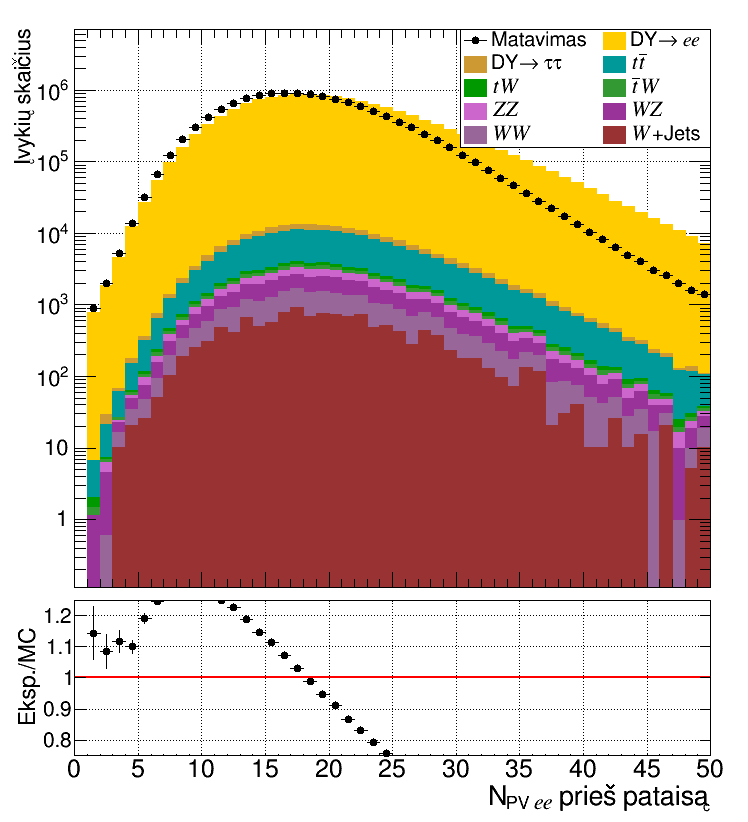
\includegraphics[width=0.48\textwidth]{nVTXee_before.png}
	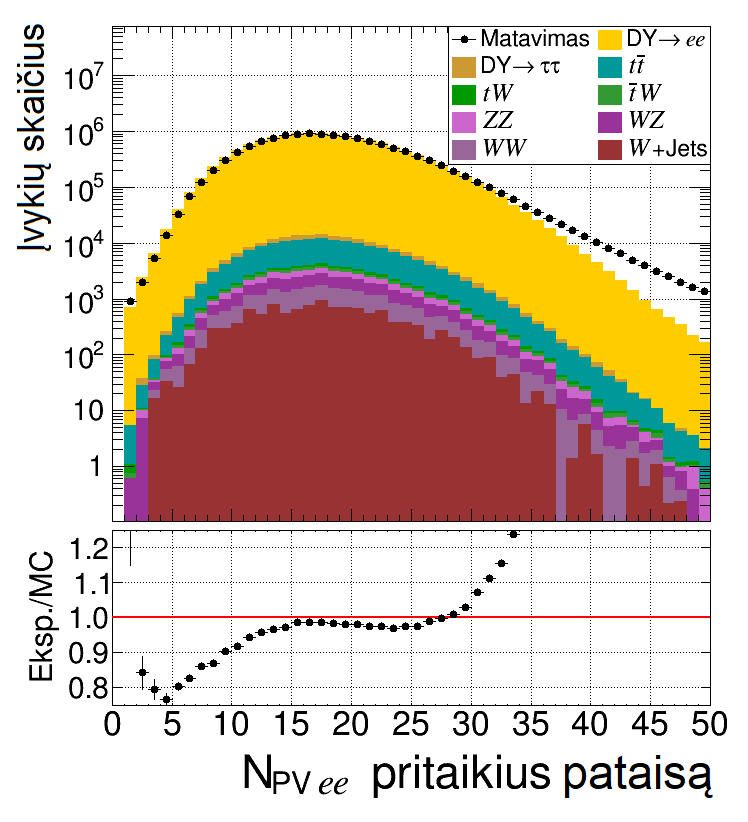
\includegraphics[width=0.48\textwidth]{nVTXee_after.png}
	\caption{\label{fig:PUba} Pirminių viršūnių skaičiaus pasiskirstymai atranką praėjusiuose elektronų poros
		įvykiuose prieš (kairėje) ir po (dešinėje) pataisos pritaikymo.
		Juodi taškai vaizduoja CMS detektoriumi išmatuotą, o spalvoti stulpeliai -- modeliuotus pasiskirstymus.}
\end{figure}

\begin{figure}[H]
	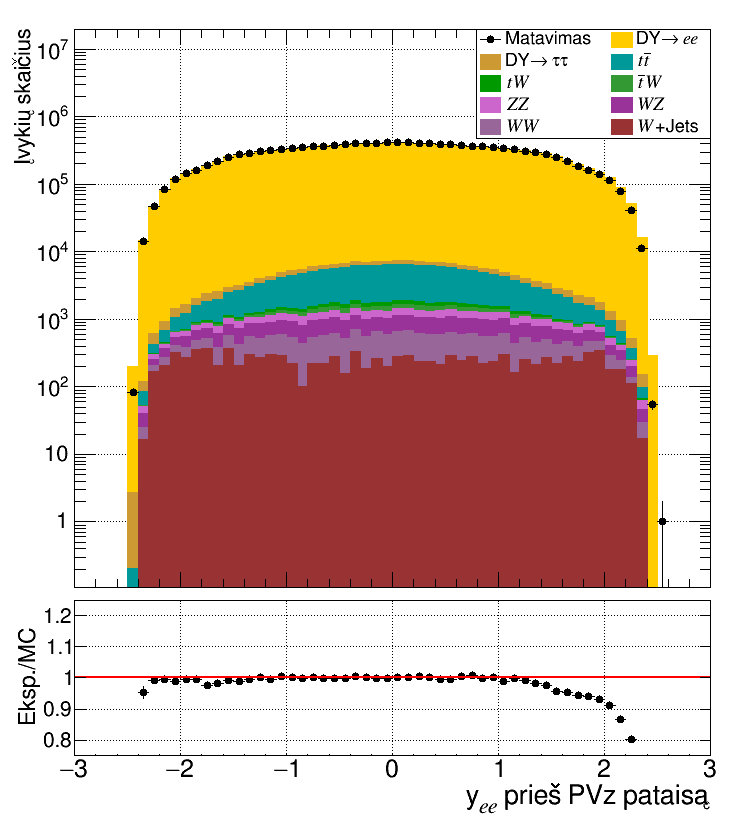
\includegraphics[width=0.48\textwidth]{ee_rapi_beforePVZ.png}
	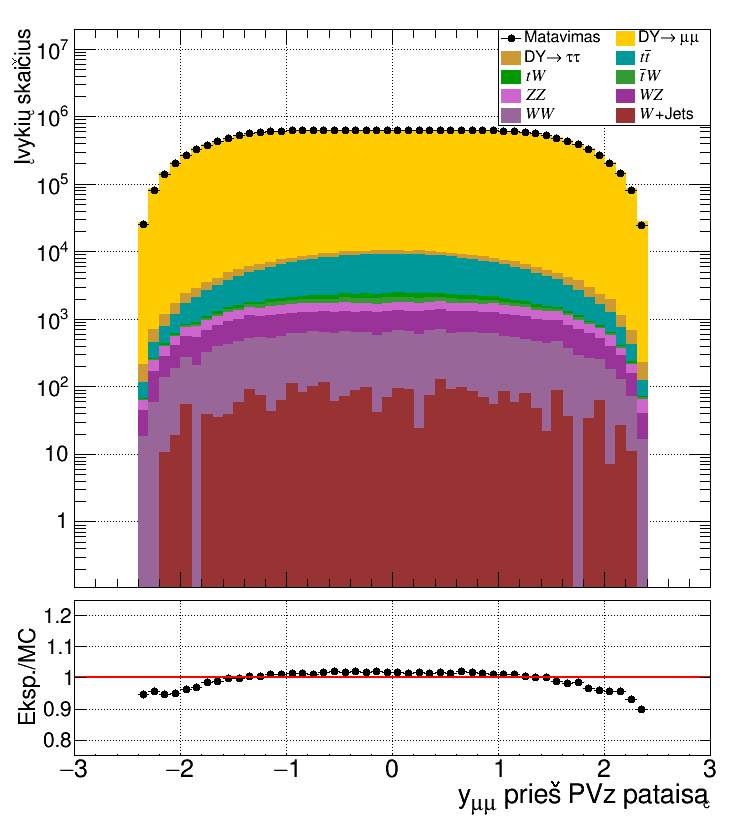
\includegraphics[width=0.48\textwidth]{mumu_rapi_beforePVZ.png}
	\caption{\label{fig:rapibPVZ} Elektronų (kairėje) ir miuonų (dešinėje) porų spartos pasiskirstymai
		prieš pirminės viršūnės (PV) $z$ koordinatės pataisos pritaikymą.
		Atkreiptinas dėmesys į eksperimento ir modeliavimo santykio pasiskirstymo asimetriškumą.}
\end{figure}

\begin{figure}[H]
	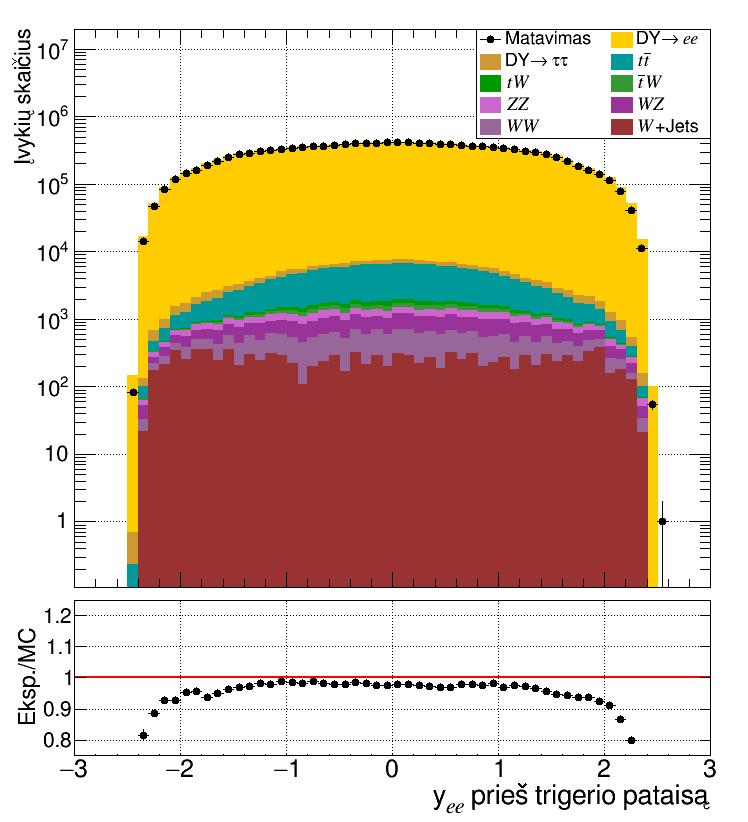
\includegraphics[width=0.48\textwidth]{ee_rapi_beforeL1.png}
	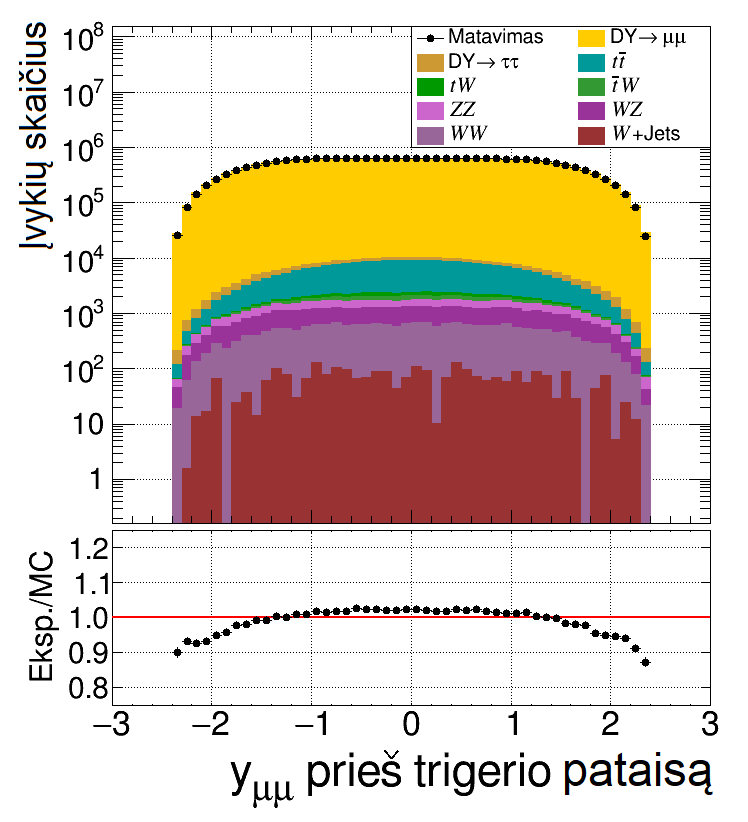
\includegraphics[width=0.48\textwidth]{mumu_rapi_beforeL1.png}
	\caption{\label{fig:rapibL1} Elektronų (kairėje) ir miuonų (dešinėje) porų spartos pasiskirstymai,
		gauti po pirminės viršūnės (PV) $z$ koordinatės pataisos pritaikymo, tačiau dar nepritaikius per ankstaus
		trigerio suveikimo pataisos.}
\end{figure}

\begin{figure}[H]
	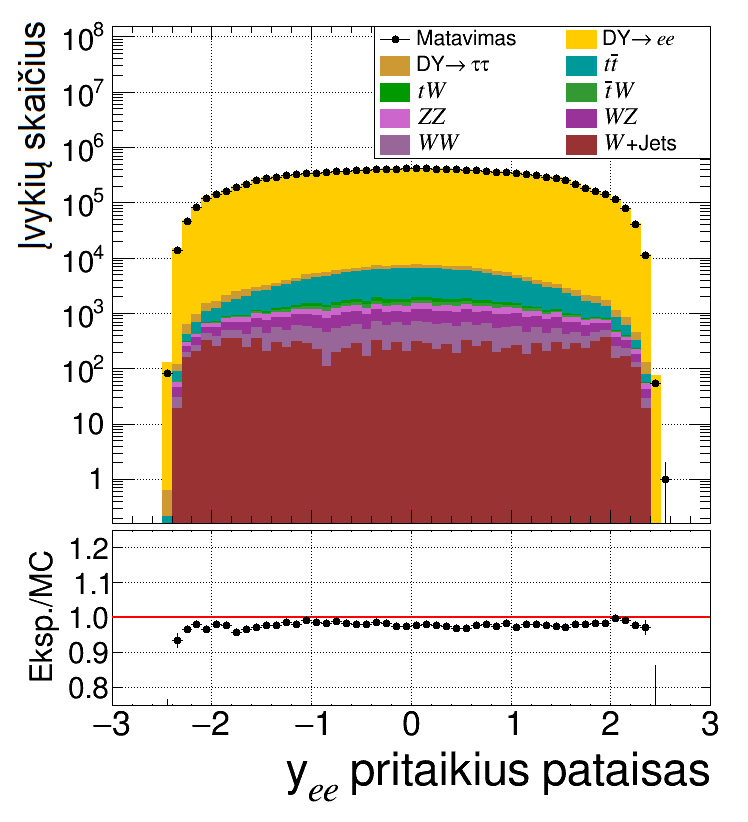
\includegraphics[width=0.48\textwidth]{ee_rapi_after.png}
	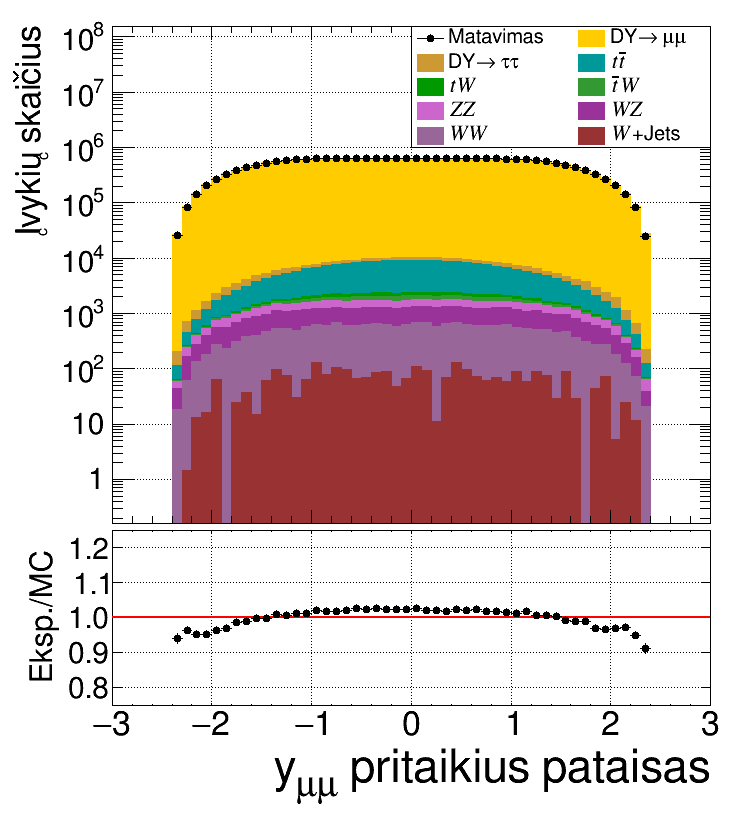
\includegraphics[width=0.48\textwidth]{mumu_rapi_after.png}
	\caption{\label{fig:rapia} Elektronų (kairėje) ir miuonų (dešinėje) porų spartos pasiskirstymai,
		gauti pritaikius visas pataisas.}
\end{figure}


Invariantinės masės pasiskirstymai prieš ir po visų pataisų pritaikymo pateikiami atitinkamai \ref{fig:invMba} pav.
Palyginus paveikslų apačioje pateikiamus matavimo ir modeliavimo santykio pasiskirstymus galima pamatyti, kad
pritaikius minėtas pataisas sutapimas tarp eksperimento ir modeliavimo pagerėjo vidutiniškai apie $10\%$.

\begin{figure}[tbp]
	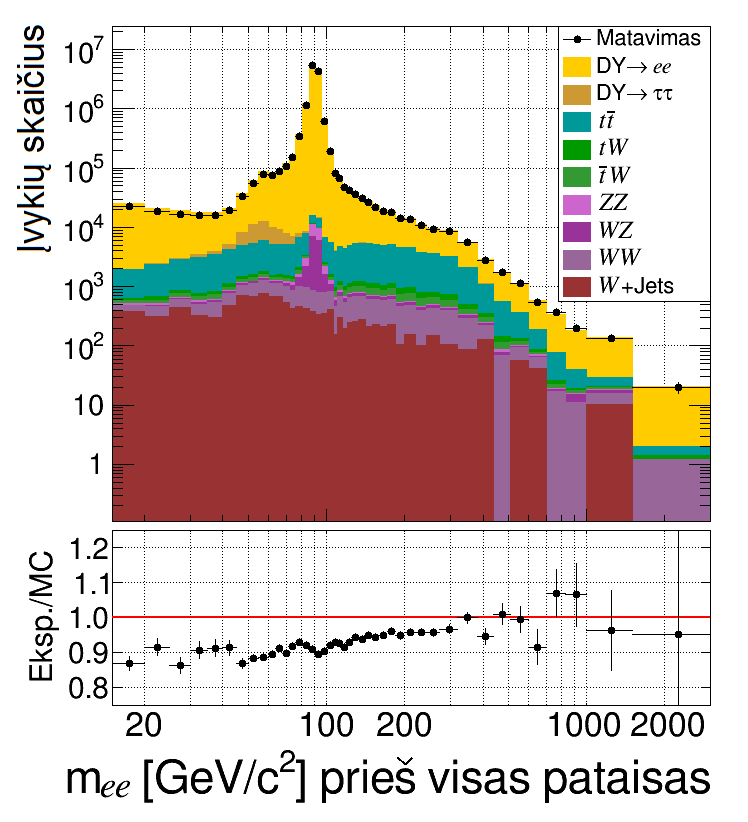
\includegraphics[width=0.48\textwidth]{ee_mass_beforeALLcorr.png}
	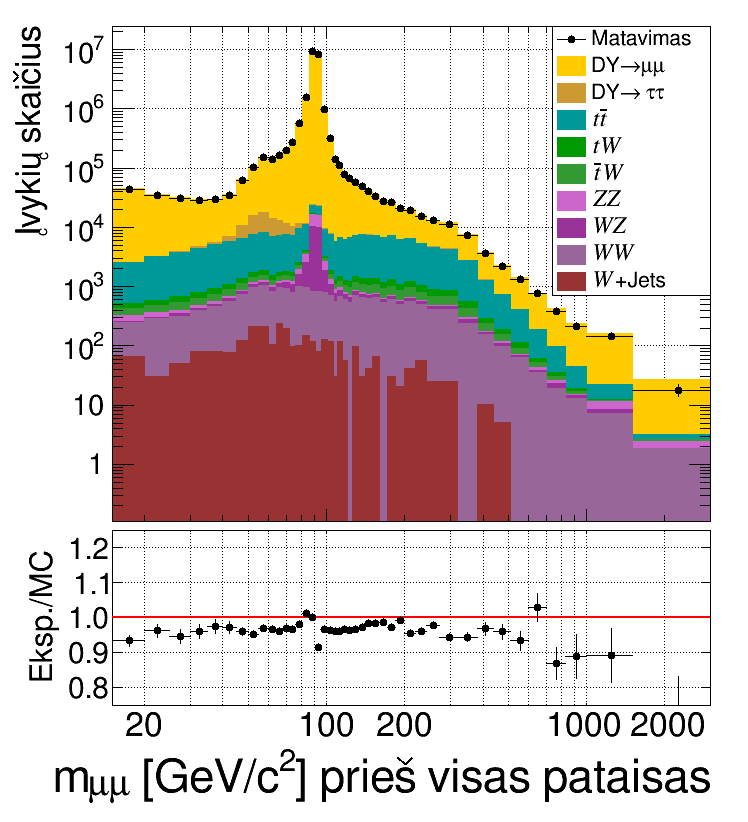
\includegraphics[width=0.48\textwidth]{mumu_mass_beforeALLcorr.png}
	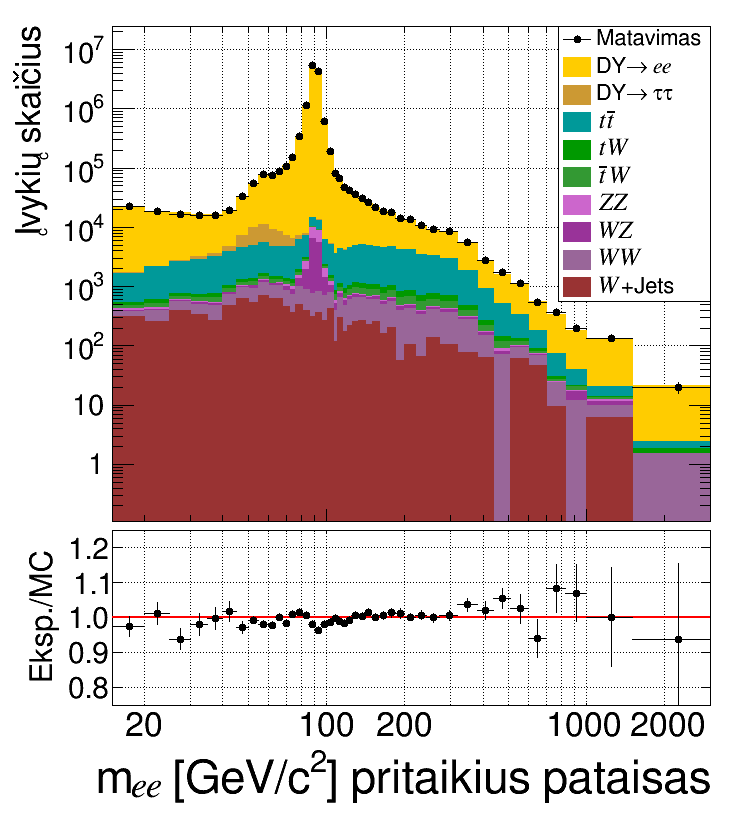
\includegraphics[width=0.48\textwidth]{ee_mass_after.png}
	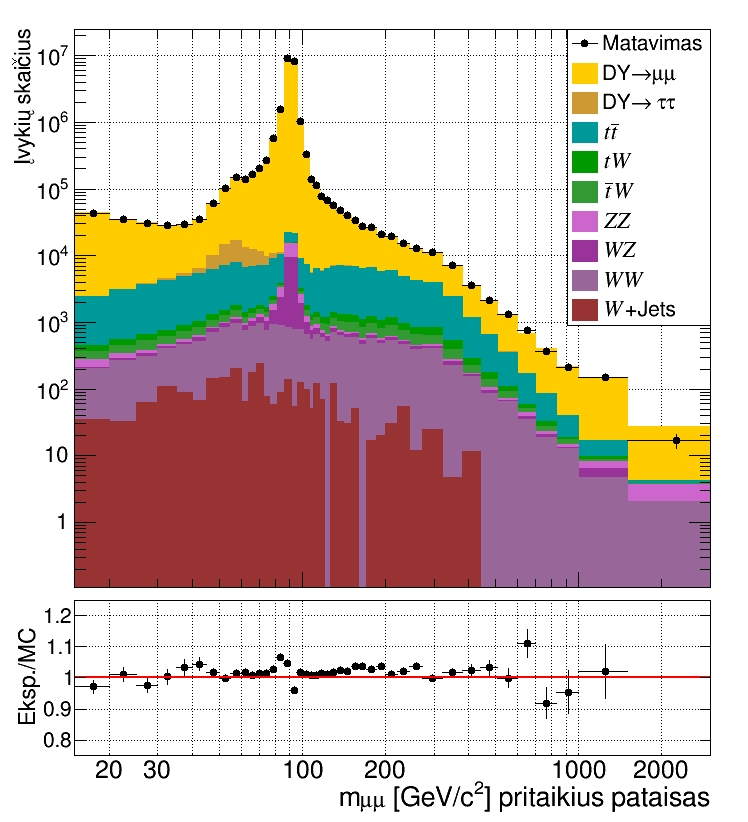
\includegraphics[width=0.48\textwidth]{mumu_mass_after.png}
	\caption{\label{fig:invMba} Elektronų (kairėje) ir miuonų (dešinėje) porų invariantinės masės pasiskirstymai
		prieš (viršuje) ir po (apačioje) efektyvumo pataisų pritaikymo.}
\end{figure}


\subsection{Drell-Yan proceso triukšmo įvykių skaičiaus įvertinimas}
Drell-Yan proceso triukšmo įvykių skaičius tiek $ee$, tiek $\mumu$ galutinėms būsenoms buvo įvertintas $\emu$
metodu ($\DYtau$, $t\bar{t}\,$, $WW$, $tW$, $\bar{t}W$ procesams) arba iš modeliavimo ($W+\mathrm{Jets}$, $WZ$,
$ZZ$ procesams).
$QCD$ triukšmo įvykių skaičius, patenkantis į $ee$ ir $\mu\mu$ sritis, kol kas dar įvertintas nebuvo, bet tam skirta metodika
jau yra paruošta ir bus naudojama tolesniame darbe.
$\emu$ metodas buvo taikomas kiekvienam histogramos stulpeliui atskirai, naudojantis \eqref{eq:emuMethod} formule.
Statistinės įvykių skaičiaus paklaidos buvo įvertintos naudojantis \eqref{eq:Sumw2Unc} ir \eqref{eq:DerUnc}
formulėmis, o sisteminės paklaidos -- naudojantis \eqref{eq:systUncEmu} formule.
Suminės paklaidos gautos susumavus statistinę ir sisteminę paklaidas pagal Pitagoro teoremą.
Triukšmo įvykių skaičiaus įverčiai, gauti $\emu$ metodu, pateikiami \ref{fig:bkgEst} pav.
Po grafikais taip pat pateikiami įverčio ir modeliavimo santykio pasiskirstymai.
Grafikuose juodi vertikalūs brūkšniai žymi statistines, o mėlynai užtušuotos juostos -- sumines įvykių skaičiaus paklaidas.
Tokio žymėjimo laikomasi visuose pateikiamuose grafikuose.
Visoje tirtoje invariantinių masių srityje susumuotas modeliuotų $ee$ triukšmo įvykių skaičius yra lygus $165031$,
o $e\mu$ metodu įvertintas $ee$ triukšmo įvykių skaičius lygus $158777$.
Modeliuotų $\mu\mu$ triukšmo įvykių skaičius lygus $250500$, o įvertinus $\mu\mu$ triukšmo įvykių skaičių  $e\mu$ metodu
gauta $241105$ įvykių.
Lyginant su modeliavimu, $\emu$ metodas visoje tirtoje invariantinės masės srityje susumuotą triukšmo įvykių skaičių
abiejuose kanaluose sumažino maždaug $4$-ais procentais.
Šis skirtumas yra sisteminė paklaida.
\ref{fig:bkgEst} pav. apačioje pateikti $\emu$ įverčio ir modeliavimo santykio grafikai atrodo taip pat
tiek $ee$, tiek $\mu\mu$ įvykiams, nes, pagal \eqref{eq:emuMethod} formulę,
$$\frac{N_{ll}^{\mathrm{Tr. \, įvert.}}}{N_{ll}^{\mathrm{Tr. \, MC}}} =
\frac{N_{\emu}^{\mathrm{Tr. \, eksp.}}}{N_{\emu}^{\mathrm{Tr. \, MC}}} \; .$$
Šis santykis yra vienodas tiek $ee$, tiek $\mu\mu$ įvykiams.
Netikrų $\emu$ įvykių įvertinimo taikant $\emu$ metodą patobulinimas įtraukiant modeliuotus $\WJets$ įvykius padėjo
sumažinti ankstesnio semestro darbe matytą didelį sisteminį nuokrypį \cite{MAk1}.
Taip pat įvertinto su $\QCD$ procesu siejamų netikrų $\emu$ įvykių skaičiaus paklaida siekia tik apie $4\%$.
Įvertinant šį skaičių modeliavimu paklaida viršija $50\%$.
Tai leidžia teigti, jog netikrų $\emu$ įvykių skaičiaus įvertinimas iš matavimo leidžia patikslinti $\emu$ metodo įvertį.
Norint šį įvertį patikslinti dar labiau, ateityje vertėtų iš matavimo įvertinti ir su $\WJets$ procesu siejamų netikrų $\emu$ įvykių skaičių.
Tam pasitarnaus klaidingo atpažinimo metodas, su kurio veikimo principu jau susipažinta.

\ref{fig:MassDataMCest} pav. pateikiamos leptonų porų invariantinių masių histogramos, kuriose $\DYtau$, $\ttbar$,
$tW$, $\tbarW$, ir $WW$ procesų modeliuoti įverčiai yra pakeisti į gautuosius naudojant $\emu$ metodą (legendoje žymima
\ltq{įvert.}).
Šie triukšmo įvykiai sudaro $1.23\%$ visų $ee$ ir $1.06\%$ visų $\mu\mu$ įvykių.
Po grafikais pateikiami matavimo ir suminio (Drell-Yan signalo, $WW$, $ZZ$ ir $W+\mathrm{Jets}$ modeliuoto ir 
$e\mu$ metodu įvertinto kitų triukšmo procesų) įverčio santykio pasiskirstymai.

Pritaikius klaidingo atpažinimo metodą bus galima gauti matavimu grįstus $\WJets$ bei $\QCD$, kuris kol kas į $ee$ ir $\mu\mu$ grafikus
nebuvo įtrauktas, įvykių skaičiaus įverčius.
Darbas bus tęsiamas bendradarbiaujant su CMS kolektyvo mokslininkais.

\begin{figure}[H]
	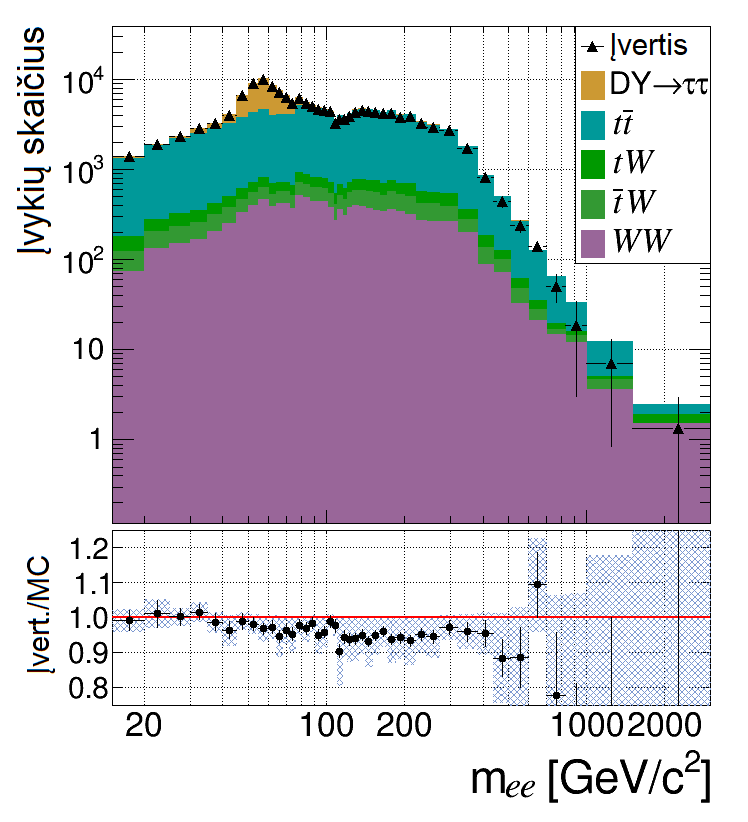
\includegraphics[width=0.49\textwidth]{ee_bkg_est.png}
	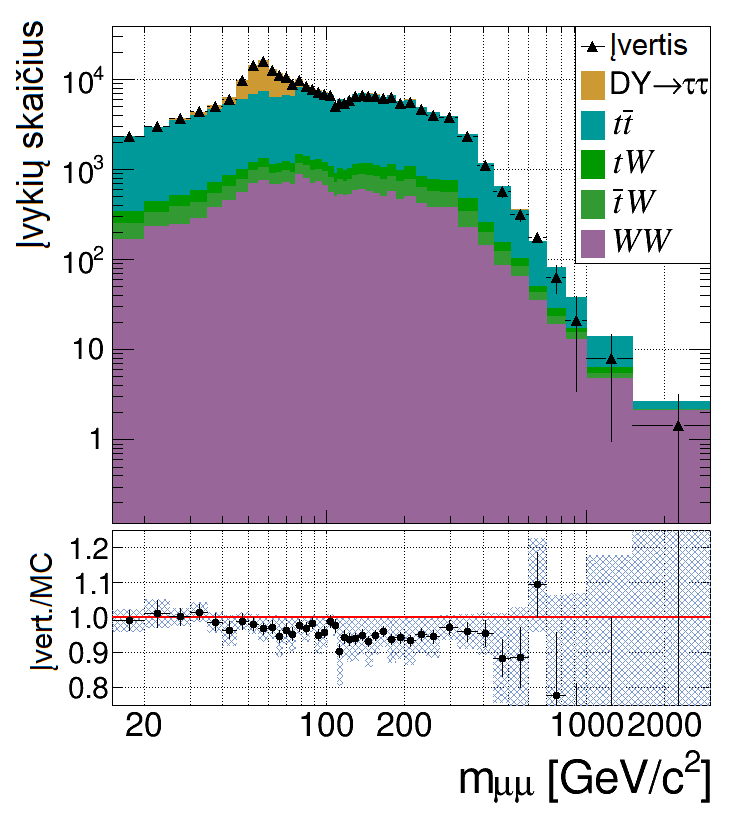
\includegraphics[width=0.49\textwidth]{mumu_bkg_est.png}
	\caption{\label{fig:bkgEst}
		Su Drell-Yan triukšmo procesais siejamų elektronų (kairėje) ir miuonų (dešinėje) porų invariantinių masių pasiskirstymai.
		Spalvoti histogramų stulpeliai vaizduoja modeliuotus, o juodi trikampiai -- $\emu$ metodu apskaičiuotus pasiskirstymus.}
\end{figure}

\begin{figure}[H]
	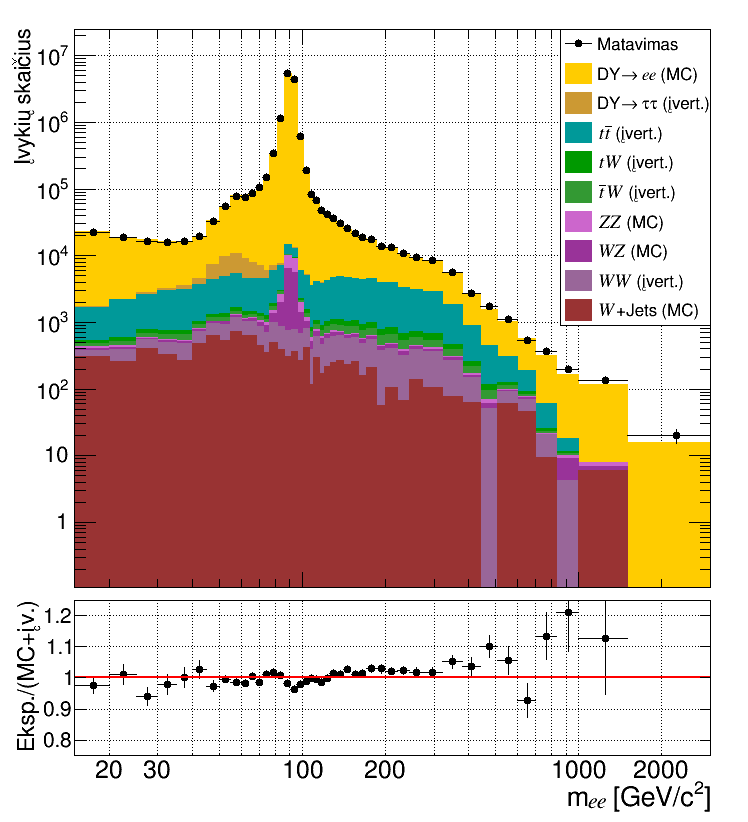
\includegraphics[width=0.49\textwidth]{ee_mass_est.png}
	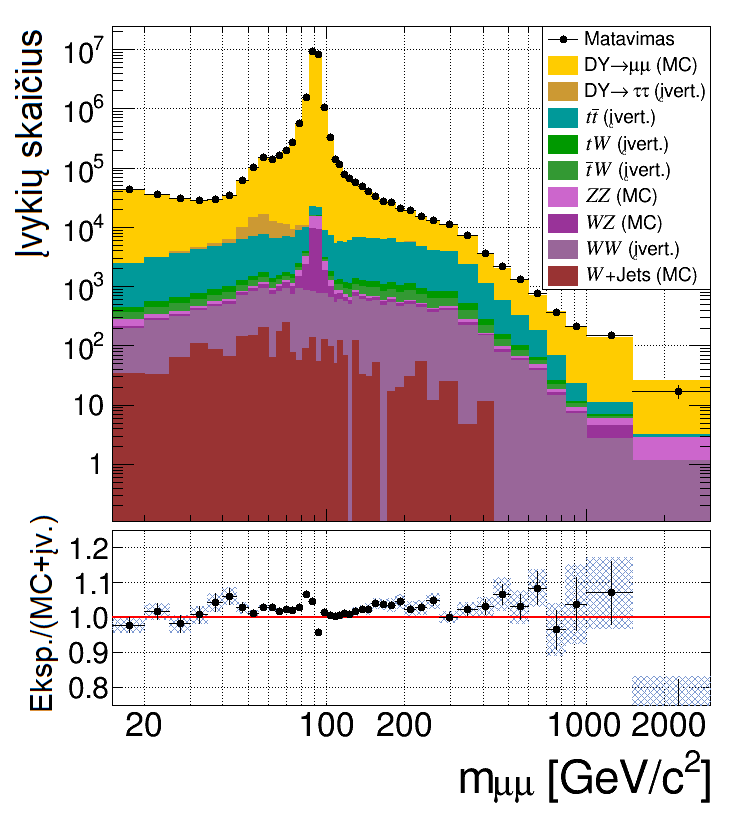
\includegraphics[width=0.49\textwidth]{mumu_mass_est.png}
	\caption{\label{fig:MassDataMCest}
		Elektronų (kairėje) ir miuonų (dešinėje) porų invariantinių masių pasiskirstymų histogramos.
		Juodi taškai vaizduoja CMS detektoriumi išmatuotą, o spalvoti stulpeliai -- modeliuotus ir $\emu$ metodu įvertintus
		pasiskirstymus.}
\end{figure}


\section{Išvados}
\begin{enumerate}
	\item Duomenų rinkinių sukūrimas, saugant tik atranką praėjusius įvykius, gerokai sutrumpina tolimesnės duomenų analizės
	laiką bei supaprastina duomenų saugojimą;
	\item Eksperimento ir modeliavimo sąlygų nesutapimų pataisos padeda sumažinti atranką praeinančių išmatuotų ir modeliuotų
	įvykių skaičiaus neatitikimus bei leidžia gauti tikslesnį $\emu$ metodo įvertį;
	\item Iš matavimo duomenų įvertinus su $QCD$ siejamų netikrų $\emu$ įvykių skaičių galima patikslinti tikrų $\emu$ įvykių
	skaičių. Dar tikslesnį rezultatą bus galima gauti iš matavimo nustačius ir su $W+\mathrm{Jets}$ procesu siejamų netikrų
	$\emu$ įvykių skaičių;
	\item $\emu$ metodas yra tinkamas Drell-Yan proceso triukšmo įvykių, kuriuose nepriklausomai sukuriami du mus dominantys
	tikri leptonai, skaičiaus įvertinimui;
	\item Drell-Yan proceso triukšmo įvykių skaičių bus galima dar labiau patikslinti įvertinus $\WJets$ ir $\QCD$ įvykių skaičių
	klaidingo atpažinimo metodu, su kurio principais jau susipažinta.
\end{enumerate}


\addcontentsline{toc}{section}{Naudotos literatūros sąrašas}
\bibliography{KursinisDarbas}
\bibliographystyle{unsrt}

%\clearpage
\section*{Santrauka}
\addcontentsline{toc}{section}{Santrauka}
\begin{center}Marijus Ambrozas \\ \textbf{Drell-Yan proceso triukšmo įvykių skaičiaus įvertinimas matavimu grįstais metodais} \end{center}

Šiame darbe pristatoma Drell-Yan proceso paieška analizuojant CERN CMS eksperimento 2016 metais užregistruotus
$13$ TeV energijos protonų susidūrimų duomenis, atitinkančius $35.9$ \invfb integruotąjį šviesį.
Paieška buvo vykdoma elektronų ir miuonų kanaluose.
Įvykdžius į Drell-Yan procesą panašių įvykių atranką buvo bandoma nustatyti, koks yra triukšmo įvykių indėlis
leptonų porų invariantinės masės pasiskirstymuose.
$\DYtau$, $\ttbar\,$, $WW$, $tW$ ir $\bar{t}W$ procesų indėliai buvo įvertinti matavimu grįstu $\emu$ metodu,
atsižvelgus į $\QCD$ ir $\WJets$ priemaišas $\emu$ įvykiuose, o $\ZZ$, $\WZ$ ir $\WJets$ indėliai buvo nustatyti
iš modeliavimo.
Pritaikius klaidingo atpažinimo metodą, kurio veikimo principas pristatomas šiame darbe, bus galima iš matavimo įvertinti
$\WJets$ ir $\QCD$ procesų įnašą į $ee$ ir $\mu\mu$ įvykių skaičių.
Elektronams ir miuonams buvo pritaikytos atitinkamai energijos ir skersinio impulso matavimo skalių pataisos.
Taip pat modeliuotiems įvykiams buvo pritaikytas rinkinys pataisų, įskaitančių įvairius neatitikimus tarp eksperimento
ir modeliavimo sąlygų.

\section*{Summary}
\begin{center} Marijus Ambrozas \\ \centering \textbf{Drell-Yan process background estimation using data-driven methods} \end{center}

The search of Drell-Yan process in $13$ TeV proton-proton collision data is presented in this work.
The data was collected in 2016 by CERN CMS experiment and corresponds to the integrated luminosity of $35.9$ \invfb.
The search was performed in electron and muon channels.
The main task of this work was to estimate the contribution of Drell-Yan background processes to dilepton invariant mass distributions.
The number of $\DYtau$, $\ttbar\,$, $WW$, $tW$, and $\bar{t}W$ background events was estimated using data-driven $\emu$ method,
after considering the $\QCD$ and $\WJets$ contamination in the $\emu$ event sample.
Contribution of $\ZZ$, $\WZ$ and $\WJets$ processes was estimated from Monte Carlo simulation.
The data-driven Fake Rate method, which is presented in this work, is going to be used to estimate the number of $\QCD$ and $\WJets$ events
in $ee$ and $\mu\mu$ channels in the nearest future.
Several corrections were used in order to get more precise results.
Energy and momentum scale correction were applied to electrons and muons respectively.
Various other corrections were applied to simulated events considering the mismatch of real and simulated experimental conditions.


\section*{Bibliografinis aprašas}
%\addcontentsline{toc}{section}{Bibliografinis aprašas}
Marijus Ambrozas. Drell-Yan proceso triukšmo įvykių skaičiaus įvertinimas matavimu grįstais metodais.
Teorinės fizikos ir astrofizikos magistro studijų antrojo semestro mokslo tiriamasis darbas.
Vad.\ Andrius Juodagalvis. Vilnius: Vilniaus universitetas, Fizikos fakultetas, 2019.
\end{document}